\documentclass[type=drfinal, dr=rernat, accentcolor=tud7b,colorbacktitle, bigchapter, openright, twoside, 12pt ]{./tudthesis}
\usepackage[english]{babel} 
\usepackage[utf8]{inputenc}
\usepackage{graphicx}
\usepackage{pstricks}
\usepackage{psfrag}
\usepackage{enumerate}
\usepackage{float}
\usepackage{epsfig}
\usepackage{subfigure}
\usepackage{rotating}
\usepackage{minitoc}
\usepackage{appendix}
\usepackage{acronym}
\usepackage{graphics}
\usepackage{amsmath}
\usepackage{multirow}
\usepackage{listings}
\usepackage[abs]{overpic}
\usepackage{pdfpages}


%%%% 1 1/2 facher Zeilenabstand:	
\usepackage{setspace}
\onehalfspacing


\setcounter{minitocdepth}{2}
\setcounter{tocdepth}{2}

% 
\thesistitle{In Silico Comparison of Photons versus Carbon Ions in Single Fraction Therapy of Lung Cancer}{In Silico Vergleich der Lungen Krebstherapie mit Photonen und Kohlenstoff Ionen bei Einzeitbestrahlung}
\author{Dipl.-Phys. Kristjan Anderle}
\birthplace{Jesenice, Slowenien}
\date{Juni 2016}
\referee{Prof. Dr. Marco Durante}{Prof. Dr. Thomas Aumann}
\department{Fachbereich Physik}
\setinstitutionlogo{GSI_Logo_cmyk}
%\department{Fachbereich Physik}
%\group{Medical Physics}
\date{Juli 2016}
\dateofexam{4. Juli 2016}{14. Juni 2016}



\begin{document}

  \makethesistitle
% \includepdf[pages={2}]{TitlePage.pdf}

\dominitoc
\setcounter{tocdepth}{1}
% 
%   \documentclass[type=dr, dr=rernat, acm$^3$entcolor=tud7b,colorbacktitle, bigchapter, openright, twoside, 12pt ]{tudthesis}
%\documentclass[11pt,twoside,a4paper]{article}
\usepackage[english]{babel} 
\usepackage[utf8]{inputenc}
\usepackage{graphicx}
\usepackage{pstricks}
\usepackage{psfrag}
\usepackage{enumerate}
\usepackage{float}
\usepackage{epsfig}
\usepackage{geometry}
\usepackage{subfigure}
\usepackage{rotating}
\usepackage{minitoc}
\usepackage{multirow}
%\usepackage{appendix}

%%%% 1 1/2 facher Zeilenabstand:	
\usepackage{setspace}
\onehalfspacing

\section*{Abstract}


Stereotactic body image guided radiation therapy (SBRT) shows good results for lung cancer treatment. However, complications can arise at the end or during the treatment. 
Better normal tissue sparing might be achieved with scanned carbon ion therapy (PT) and hence reduce the number of complications. Therefore an in silico trial was conducted to find potential advantages of PT in treating lung cancer. 
A study was conducted on patients that were treated with SBRT at Champalimaud Center for the Unknown, Lisbon (Portugal). PT plans were calculated on 4D-CTs with different breathing motion patterns simulated. For successful simulation
deformable image registration was used and a tool to provide its quality assurance has been developed. 
The results of the study showed that target coverage was was the same in SBRT and PT, while PT delivered less dose to OAR. Additionally, motion was successfully mitigated with resanning. 
A special investigation was made into patients with multiple lung lesions, where PT seemed even better suited for treatment than SBRT.



\section*{Zusammenfassung}


%   
%   % \documentclass[type=dr, dr=rernat, accentcolor=tud7b,colorbacktitle, bigchapter, openright, twoside, 12pt ]{tudthesis}
% \usepackage[english]{babel} 
% \usepackage[utf8]{inputenc}
% \usepackage{graphicx}
% \usepackage{pstricks}
% \usepackage{psfrag}
% \usepackage{enumerate}
% \usepackage{float}
% \usepackage{epsfig}
% %\usepackage{geometry}
% \usepackage{subfigure}
% \usepackage{rotating}
% \usepackage{minitoc}
% \usepackage{appendix}
% 
% %%%% 1 1/2 facher Zeilenabstand:	
% \usepackage{setspace}
% \onehalfspacing
% 
% 
% \begin{document}

\newpage
\chapter*{Publications related to this work}


\section*{Article in revision}
\begin{setlength}{\leftmargini}{3ex}
 \begin{description}
 \item[] \textbf{Anderle K.}, Stroom J., Pimentel J., Greco C., Durante M. and Graeff C.: In Silico Comparison of Photons versus Carbon Ions in Single Fraction Therapy of Lung Cancer; revision under review in \textit{Phys.Med.}, submitted in March 2016 
%     \item[] Sonnabend K, Savran D, Beller, J, B\"ussing, MA, \textbf{Constantinescu A}, Elvers M, Endres J, Fritzsche M, Glorius J, Hasper J, Isaak J, L\"oher B, M\"uller S, Pietralla N, Romig C, Sauerwein A, Schnorrenberger L, W\"alzlein C, Zilges A, Zweidinger M; The Darmstadt High-Intensity Photon Setup (DHIPS) at the S-DALINAC; Nuclear Inst. and Methods in Physics Research, A; Volume 640; issue 1; p. 6-12; (2011) 
%      \item[] Seregni M, Kaderka R, Fattori G, Riboldi M, Pella A, \textbf{Constantinescu A}, Saito N, Durante M, Cerveri P, Bert C, Baroni G: Tumor tracking based on correlation models in scanned ion beam therapy: an experimental study; \textit{Phys Med Biol}; 58(13); 2013
%      \item[] Graeff C, \textbf{Constantinescu A}, L\"uchtenborg R, Durante M, Bert C: Multigating: 4D optimized beam tracking in scanned ion beam therapy; \textit{Technol Cancer Res Treat.}; Epub ahead of print DOI: 10.7785/tcrtexpress.2013.6002772013; 2013
%      \item[] Fattori G, Saito N, Seregni M, Kaderka R, Pella A, \textbf{Constantinescu A}, Riboldi M, Steidl P, Cerveri P, Bert C, Durante M and Baroni G: Commissioning of an integrated platform for time-resolved treatment delivery in scanned ion beam therapy by means of optical motion monitoring; \textit{Technol Cancer Res Treat.}; Epub ahead of print DOI: 10.7785/tcrtexpress.2013.600275; 2013
%      \item[] Lehmann HI, Richter D, Prokesch H, Graeff C, Prall M, Simoniello P, Fournier C, Bauer J, Kaderka R, Weymann A, Szabo G, Sonnenberg K, \textbf{Constantinescu A}, Johnson SB, Haberer T, Debus J, Durante M, Bert C and Packer DL: AV node Ablation in Langendorff-perfused Porcine Hearts Using Carbon Ion Particle Therapy: Methods and an In vivo Feasibility Investigation for Catheter-free Ablation of Cardiac Arrhythmias; submitted to \textit{Circulation}; April 2014
 \end{description}
\end{setlength}

\section*{GSI scientific report}
\begin{setlength}{\leftmargini}{3ex}
  \begin{description}
%     \item[] \textbf{Constantinescu A}, Saito N, Chaudhri N, Durante M, Bert C: Optimisation of the ion optical range adaptation method for tracking of moving tumours with scanned ion beams; \textit{GSI Scientific Report 2009}, 502
%     \item[] \textbf{Constantinescu A}, Saito N, Chaudhri N, Durante M, Kraft G, Bert C: Optimisation of an ion optical range adaptation method for beam tracking of moving tumours with scanned ion beams;  \textit{GSI Scientific Report 2010}, 487
    \item[] \textbf{Anderle K.}, Stroom J., Pimentel J., Greco C., Durante M. and Graeff C.: An in silico Trial of X-rays vs Carbon Ions in Single Shot Lung Cancer Therapy; \textit{GSI Scientific Report 2013}, 228
  \end{description}
\end{setlength}

%\section*{Articles}
%\begin{setlength}{\leftmargini}{1.4em}
%  \begin{description}
%    \item[] Tami Freeman: Carbon ions tackle atrial fibrillation; medicalphysicsweb.org; June 20; 2013
%      \end{description}
%\end{setlength}


\section*{Conference contributions}
\begin{setlength}{\leftmargini}{1.4em}
  \begin{description}
  %	PTCOG, 4D Workshop, ESTRO, PTCOG, DGMP, PTCOG (Anna) ESTRO (Sandra)
    \item[] \textbf{Anderle K.}, Stroom J., Pimentel J., Greco C., Durante M. and Graeff C. (2013). An in silico Comparison of Scanned Carbon Ion vs. SBRT Single Dose Treatment of Metastatic Lung Cancer; \textit{4D Treatment planning workshop}. Poster presentation
    \item[] \textbf{Anderle K.}, Stroom J., Pimentel J., Greco C., Durante M. and Graeff C. (2014). An in silico Comparison of Single Fraction Scanned Carbon Ion vs. SBRT in Metastatic Lung Cancer; \textit{ESTRO}. Poster presentation
    \item[] \textbf{Anderle K.}, Stroom J., Pimentel J., Greco C., Durante M. and Graeff C. (2015). In Silico Trial of Photons versus Carbon Ions in Single Fraction Therapy of Lung Cancer; \textit{PTCOG}. Poster presentation
    \item[] \textbf{Anderle K.}, Stroom J., Pimentel J., Greco C., Durante M. and Graeff C. (2015). In Silico Trial of Photons versus Carbon Ions in Single Fraction Therapy of Lung Cancer; \textit{DGMP}. Poster presentation
    \item[]  Prall M., Hild S., \textbf{Anderle K.} and Graeff C. (2016). Treatment Planning with an Adaptive Dose Grid; \textit{PTCOG}. Poster presentation
    \item[]  Eichhorn A., Hild S., \textbf{Anderle K.} and Graeff C. (2016). Speed-up of plan delivery for intensity modulated particle therapy by splitting iso-energy slices according to beam intensity levels; \textit{PTCOG}. Poster presentation
    \item[]  Vieira S., Stroom J., \textbf{Anderle K.}, Salas B., Pimentel N. and Greco C. (2016). Validation of freeware-based midventilation CT calculation for upper abdominal cancer patients; \textit{ESTRO}. Poster presentation
    
    
    
      \end{description}
\end{setlength}




% \end{document}
% 
%   \tableofcontents
%   
%   % \documentclass[type=dr, dr=rernat, accentcolor=tud7b,colorbacktitle, bigchapter, openright, twoside, 12pt ]{tudthesis}
% \usepackage[english]{babel} 
% \usepackage[utf8]{inputenc}
% \usepackage{graphicx}
% \usepackage{pstricks}
% \usepackage{psfrag}
% \usepackage{enumerate}
% \usepackage{float}
% \usepackage{epsfig}
% %\usepackage{geometry}
% \usepackage{subfigure}
% \usepackage{rotating}
% \usepackage{minitoc}
% \usepackage{appendix}
% % \usepackage{epstopdf}
% \usepackage{graphics}
% 
% \usepackage{acronym}
%  
% %%%% 1 1/2 facher Zeilenabstand:	
% \usepackage{setspace}
% \onehalfspacing



% \begin{document}
 

\twocolumn
\chapter*{List of Abbreviations}


\begin{acronym}[MDACC]
\setlength{\itemsep}{-\parsep}
% \setlength{\parsep}{0.5cm}

  \acro{3DCRT}{three dimensional conformal radiotherapy}
  \acro{4D-CT}{time resolved computed tomography}
  \acro{4Dopt}{time resolved optimization}
  \acro{AP}{anterior-posterior}
%   \acro{COPD}{chronic obstructive pulmonary disease}
%   \acro{CiT}{scanned carbon-ion therapy}
  \acro{CNAO}{National Centre of Oncological Hadrontherapy, Pavia, Italy}
  \acro{CT}{computed tomography}
  \acro{CTV}{clinical target volume}
%   \acro{Cx43}{Connexin 43}
%   \acro{D5-D95}{measure for dose homogeneity}
 \acro{$D_{99}$}[$D_{99\%}$]{minimum dose delivered to 99\% of volume }
 \acro{$D_{Max}$}{maximum dose delivered to a single voxel }
 \acro{$D_{Mean}$}{mean dose delivered to volume}
  \acro{DIR}{deformable image registration}
  \acro{DIRQA}{quality assurance of deformable image registration}
%   \acro{DKFZ}{Deutsches Krebsforschungszentrum}
  \acro{DNA}{deoxyribonucleic acid}
  \acro{DSB}{double strand breaks}
  \acro{DVH}{dose volume histogram}
  \acro{FWHM}{full width at half maximum}
  \acro{GSI}{GSI Helmholtzzentrum f\"ur Schwerionenforschung GmbH}
  \acro{GTV}{gross tumor volume}
%   \acro{GyE}{Gray equivalent}
  \acro{HIT}{Heidelberg Ion-Beam Therapy Centre}
  \acro{HU}{Hounsfield unit}
  \acro{ECG}{electrocardiography}
  \acro{IES}{iso-energy slice}
%   \acro{IM}{internal margin}
  \acro{IMPT}{intensity modulated particle therapy}
%  \acro{IMPT(OAR)}{IMPT with included OAR}
  \acro{IMRT}{intensity modulated radiotherapy}
  \acro{ITV}{internal target volume}
%   \acro{IVC}{inferior vena cava}
%   \acro{LAA}{left atrial appendage}
%   \acro{LAB}{left atrial body}
  \acro{LEM}{local effect model}
  \acro{LET}{linear energy transfer}
  \acro{LR}{left-right}
  \acro{MLC}{multileaf collimators}
%   \acro{MP}{motion phase}
  \acro{MRI}{magnetic resonance imaging}
  \acro{NIRS}{National Institute of Radiological Sciences, Chiba, Japan}
  \acro{noPM}{no pacemaker}
  \acro{OAR}{organ at risk}
  \acro{PET}{positron emission tomography}
  \acro{PM}{pacemaker}
  \acro{PMMA}{polymethyl methacrylate}
  \acro{PSI}{Paul Scherrer Institut}
  \acro{PTV}{planning target volume}
  \acro{RBE}{relative biological effectiveness}
  \acro{RTOG}{Radiotherapy Oncology Group}
  \acro{SA}{smaller airways}
  \acro{SI}{superior-inferior}
  \acro{SBRT}{stereotactic body radiation therapy}
  \acro{SDRT}{single dose radiotherapy}
  \acro{SFUD}{single field uniform dose}
  \acro{SOBP}{spread out Bragg peak}
  \acro{SSB}{single strand break}
%   \acro{SVC}{superior vena cava}
  \acro{TRiP}{treatment planning for carbon ion radiotherapy}
 \acro{$V_{20}$}[$V_{20\%}$]{volume which received at least 20\% of the target dose (dose coverage)}
%   \acro{$V_{99\%}$}{volume which received at least 99\% of the target dose (dose coverage)}
 % \acro{$V_{107\%}$}{volume which received at least 107\% of the target dose (over dosage)}
  \acro{VMAT}{volumetric modulatec arc therapy}
\end{acronym}
\onecolumn

% \end{document}

% 
%   \documentclass[type=dr, dr=rernat, accentcolor=tud7b,colorbacktitle, bigchapter, openright, twoside, 12pt ]{tudthesis}
%\documentclass[11pt,twoside,a4paper]{article}
\usepackage[english]{babel} 
\usepackage[utf8]{inputenc}
\usepackage{graphicx}
\usepackage{pstricks}
\usepackage{psfrag}
\usepackage{enumerate}
\usepackage{float}
\usepackage{epsfig}
\usepackage{geometry}
\usepackage{subfigure}
\usepackage{rotating}
\usepackage{minitoc}
% \usepackage{dominitoc}
\usepackage{multirow}
\usepackage{listings}
%\usepackage{appendix}
%\usepackage[breaklinks=true]{hyperref}
%\usepackage{breakcites}

%%%% 1 1/2 facher Zeilenabstand:	
\usepackage{setspace}
\onehalfspacing


%chapter*{Motivation}
%\addcontentsline{toc}{chapter}{Motivation}

\section*{Motivation}

In 2013 every fourth death in Germany was due to cancer \cite{Destatis2015} and approximately 45 000 of deaths were from lung and bronchial cancer. In the last 30 years, there was a 180\% increase of deaths due to lung and bronchial cancer for women \cite{Destatis2015}.
The standard course of treatment for lung cancer is surgery, chemotherapy, radiotherapy or a combination of these. Surgery is usually the first choice of treatment. In recent years, however, state of the art photon radiotherapy, called stereotactic body-radiation therapy (SBRT) showed
promising results for treating lung cancer \cite{Baumann2009, Greco2011}. SBRT delievers high doses (up to 24 Gy) in few fractions, therefore a careful consideration must be given to dose to critical structures.

In the last twenty years, ion beam therapy has proven to be an alternative to photon radiotherapy. Higher tumor control rates and better dose conformity can be achieved with superior physical and biological properties of ions \cite{Tsujii2008,Durante2010}.
Review made by Kamada et al reported a high 3-year survival rate for carbon-ions (76.9\%) in single fraction, with no late treatment-related complications \cite{Kamada2016}. The treatment used passive beam scanning, where patient specific absorbers are used to conform the dose
to the tumor. Active beam scanning can provide better dose shaping, which is essential in hypo-fractionated treatment. However, interaction between tumor and scanned beam motion, called interplay, can severely degrade dose distribution in patient.

Successful treatment of tumors in abdomen region with scanned ion beams has been done in CNAO and NIRS. None, however, have treated lung cancer patients, where range changes between soft (lung) and dense (tumor) tissue can be substantial, making treatment planning and delivery of 
scanned ion beam a challenging problems.

In this thesis we will address this challanges and make a comparison between SBRT and scanned carbon-ion therapy. Patients particulary suited for carbon-ion therapy will try to be identified for a possible future treatment at facilities in HIT or Marburg. 



\newpage

\section*{Scope of this work}

This is the first in silico comparision between SBRT and active scanning carbon-ion for NSCLC. Time-resolved (4D) doses will be studied on a large patient dataset.

In order to create carbon-ion treatment plans and calculate 4D doses, contours have to be propagated from planning to all states 4D computed tomography (CT) and motion between 4D-CT states has to be quantified. 
This will be achieved with deformable image registration (DIR). 
Furthermore, a designated tool for DIR quality assurance (DIRQA) will be developed. A verification of DIR and DIRQA has been done on human lung 4D-CT and on pig cardiac 4D-CT.

To show potential of scanned carbon-ions in handling NSCLC, treatment plans for 19 patients, which were treated with SBRT, will be calculated. Furthermore, static and 4D doses with and without motion
mitigation will be analyzed. Doses to target and organs-at-risk (OAR) will be analyzed and compared between carbon-ions and SBRT.

A special investigation will be made into patients with multiple NSCLC metastases. A treatment planning software will be modified, so it will be able to make treatment plans for multiple targets. 
Treatment plans for patients with multiple NSCLC metastases will be generated with two different optimization techniques to tackle range changes in moving targets. Comparison to SBRT will be made regarding target coverage and OAR doses.

The structure of this dissertation is as follows. Chapter 1 will present an overview of physical and biological fundamentals of radiotherapy. Photon and particle radiotherapy will be presented, with an emphasis on the treatment of moving targets.
Additionally, lung cancer, epidemiology and staging used will be presented. Chapter 2 will present tools to handle DIR and DIRQA with their verification. In chapter 3, comparison between SBRT and carbon-ions will be investigated on lung cancer patient.
Treatment for patients with multiple metastases in lung will be investigated in chapter 4. Overall results will be discussed in chapter 5 and the thesis will be concluded in chapter 6.



\bibliographystyle{apalike}
\bibliography{../ref.bib}{}
% \bibliographystyle{plain}

\end{document}

%   
%   \setcounter{mtc}{1}
%   \include{Fundamentals/Fundamentals_main}
%   
%   \setcounter{mtc}{2}
%   \chapter{Deformable Image Registration and Validation}
\label{chapter:vmm}
\minitoc

\section{Introduction}

%As explained in Section \textbf{ref!}, effects of motion can have a significant impact on a radiation treatment. There are several motion mitigation techniques available that can operate on beam delivery, patient immobilization or treatment planning level.

Today most modern clinics regularly use different imaging techniques including CT, 4D-CT, cone-beam CT, MRI and PET. A registration is needed to overlay different image acquisitions, such as images taken at different days,
between different imaging modalities or to quantify anatomical changes in a time-resolved image acquisition, such as 4D-CT, 4D-MRI or 4D ultra sound. While most commercial treatment planning software provide rigid registration between different images, deformable image registration (DIR) is currently rarely used. 
DIR can quantify anatomical and biological variations better compared to rigid registration \cite{Sarrut2006}. It opens exciting new options in radiotherapy, such as 4D optimization \cite{Trofimov2005}, 
4D dose calculation \cite{Flampouri2006} or contour propagation \cite{Lu2006b}. 4D dose calculation has been well established for photons \cite{Ong2016}, protons \cite{Paganetti2005} and carbon-ions \cite{Gemmel2011} and has received
several experimental verifications \cite{Vinogradskiy2009, Perrin2016, Bert2012a}. 

A 4D dose calculation requires DIR for the deformation of the dose distributions in each motion state
to the reference state, where the dose from all motion states is accumulated. 4D dose calculation requires accurate DIR at every voxel, since errors in DIR can significantly alter the 4D dose \cite{Heath2006}. Special consideration has to be paid to calculation of biological 4D doses \cite{Gemmel2011}. 

Contours can be propagated in two ways - either with DIR \cite{Lu2006a, Rietzel2005a} or
with deformable model driven techniques \cite{McInerney1996}, which uses a physical model to iteratively match the contour to image features. In contrast to a 4D dose calculation, contour propagation requires accurate DIR at the contour boundaries.

Besides radiotherapy, DIR is used also in other medical fields \cite{Cleary2010, Herrell2012, Nithiananthan2011, Naini2010}.
Several different DIR algorithms are available, such as B-spline \cite{Rueckert1999}, Demons \cite{Thirion1998}, linear elastic finite element \cite{Venugopal2005}, optical flow \cite{Zhong2007} or viscous fluid \cite{Christensen1996}.
	
The DIR has a large degrees of freedom and as such is an ill-posed problem and hence prone to errors. The errors can result in image misalignments or in physically impossible vector fields. 
One of the reasons why DIR is not commonly used in commercial softwares is the lack of proper DIR quality assurance (DIRQA), which is essential for implementation of DIR in the clinical work-flow. While several different DIRQA methods exist, none of them are definitive and most of them are time consuming. 
It is possible to evaluate DIR with deformable phantoms, where the type and size of deformation is known \cite{Kashani2007, Kirby2011}. However this effort is prohibitive 
in the everyday clinical work flow. DIR validation can also be based on landmark positions, specifically their location before and after registration. In absence of externally planted markers, locating landmarks in the patient 
anatomy can be time-consuming and it can be difficult to identify landmarks in low-contrast regions \cite{Varadhan2013}. Another option is to compare delineated contours with the propagated ones using the dice similarity coefficient \cite{Varadhan2013} or Hausdorff distance \cite{Huttenlocher1993}. 
While more efficient than landmark checks, these techniques require additional delineation and do not address the region within the contour.

A set of tools was created to systematically handle DIR and DIRQA in the open-source software 3D Slicer. Tools were tested on a large data set to verify their validity.

\newpage
\section{Implementation}
\label{Implementation}

\subsection{3D Slicer}
\label{Slicer}

3D Slicer (Slicer) is a software platform for the analysis and visualization of medical images \cite{Slicer, Fedorov2012}. Slicer is a free, open-source software (BSD-style license) available on Windows, MacOSX and Linux operating systems. 
It comes with a vast variety of tools, such as:

\begin{itemize}
	\item Handling all commonly image formats, including DICOM, NRRD and MHA
	\item Visualization of voxel images, polygonal meshes and volume renderings
	\item Image registration (rigid and non-rigid) and display of vector fields
	\item Automatic image segmentation
	\item Analysis and visualization of diffusion tensor image data
	\item Device tracking for image-guided procedures
\end{itemize}

The source code of Slicer is written in C++ and with a Python wrapper to provide rapid, iterative development. The graphical user interface is based on Qt. The visualization is based on VTK \cite{Vtk}, a graphical library commonly
used in scientific research.

Slicer is a research tool and as such allows implementation of new functionalities in the form of extensions (modules). They can either be as external command-line programs, 
as scripts to automate Slicer processes or as unique modules with new features. 

\subsection{Registration}
\label{RegistrationImplement}

Plastimatch \cite{Shackleford2010} is a commonly used software for registration in medical research. It is a free and open-source tool, available as a command-line executable program. 
Plastimatch B-spline registration is also available in Slicer as part of the extension SlicerRT \cite{Pinter2012}.
The integration of Plastimatch in Slicer brings the advantage of a graphical user interface, offering a quick modification of parameters and visualization of the results. 
However, automation is needed for a large number of registrations. For a complete 4D-CT registration there are $2(N-1)$ registrations required - from the reference phase to each of $N$ motion states of 4D-CT and vice versa, except for the reference phase itself. 
Typical 4D-CTs consist of 10 phases, therefore automated registration of a 4D-CT is necessary.

The automated DIR was achieved with a Python class to handle image locations, store DIR parameters, perform DIR in the Plastimatch module, use correct naming conventions and store all output files (vector fields and warped images). 
Details can be found in Appendix~\ref{AppendixA}.



\subsubsection{Registration nomenclature}

To provide a clear and consistent description of methods used, an overview of the expressions is given here.

\begin{itemize}
 \item \textbf{Reference image} - the image that serves as a reference position in registration (image that is being registered to).
 \item \textbf{Moving image} - the image that is matched to the reference image (image that is being registered from).
 \item \textbf{Warped image} - the result of applying a transformation map from registration to the moving image. It should be as close to the reference image as possible.
 \item \textbf{True registration} - the registration from the moving to the reference image. Similar, everything connected to the true registration will use ``true'' (true vector field, true warped image, true absolute difference, true Jacobian, etc.).
 \item \textbf{Inverse registration} - the registration from the reference to the moving image (opposite or inverse of the true registration). As in the true registration, the term inverse can be used for everything connected to it (inverse vector field, inverse warped image, inverse absolute difference, inverse Jacobian, etc.).
\end{itemize}

In radiotherapy the true registration is used for dose propagation and consequential the 4D Dose calculation, whereas with the inverse registration contours can be propagated from the reference to the moving phase.


\subsection{Registration Quality Checks}
\label{DIRQA}

In order to provide visual and quantitative assessment of the registration quality a \textbf{Deformable Image Registration Quality Assurance} or DIRQA module was created. 
It provides image checks (inverse color, checkerboard, absolute difference, flicker, movie and landmark distances) 
and vector checks (Jacobian and inverse consistency error). 
The reference and warped image, true and inverse vector are used as inputs for the DIRQA module. 
Additionally, landmarks and a region of interest (ROI) can also be used as an input.

Tests can be divided into two groups: qualitative (inverse color, checkerboard, flicker, movie) and quantitative 
(absolute difference, landmark distances, Jacobian and inverse consistency error) tests.
Absolute difference, Jacobian and inverse consistency error tests
were build using tools from the ITK library \cite{Yoo2002}.

\subsubsection{Qualitative tests}

A DIR quality can be assessed with visual inspection of DIR results. Several tests were developed to make the visual inspection easier.


\subsubsection{Inverse color}


Overlaying two different images will highlight the difference between them. However, since CT scans are usually displayed in grayscale color code, the differences can be indistinguishable. 
Especially if the images are quite similar, as the reference and the warped image should be. With applying opposite color codes to overlaying images two things are achieved. 
First, regions where the registration was successful will be in grayscale. Second, the differences between images will be highlighted in the color of the image they originate from. 
In the module we used red and cyan color code for reference and warped image, respectively. See Fig.~\ref{falseColor} for details.

\begin{figure}[H]
	\begin{center}		
		\includegraphics[width=0.9\textwidth]{./Vmm/Images/falseColor.png}
		\caption{An example of a inverse color overlay. Images (a) and (b) show red and cyan color code, respectively, for a CT scan. (c) displays overlayed inverse colored images before and (d) after registration.}
		\label{falseColor}
	\end{center}
\end{figure}

\subsubsection{Checkerboard}

As the name suggests, checkerboard creates an image of tiles. Each tile alternates between the reference and the warped image, as shown in Fig.~\ref{checkerboard}. The differences between two images become apparent if there is no smooth transition from one tile to the next. 
The number of tiles can be manually selected.
\newpage
\begin{figure}[H]
	\begin{center}		
		\includegraphics[width=0.9\textwidth]{./Vmm/Images/checkerboard.png}
		\caption{An example of a checkerboard image. It consists of tiles alternating between two images. Tiles in image (a) alternate between scans before registration and in image (b) after registration.}
		\label{checkerboard}
	\end{center}
\end{figure}

\subsubsection{Movie}

Medical images are usually quite large - a typical CT image consist of $512 \times 512 \times 100$ pixels, which makes inspecting image checks (inverse color, checkerboard, absolute difference) a time-consuming task. 
The movie feature allows a smoother display of different image slices. 
The user selects which view to inspect (axial, sagital or coronal) and presses start. Selected views then start scrolling from the first to the last slice of selected view. It allows user to focus on registration details, rather than scrolling through slices.



\subsubsection{Flicker}

While it is possible to display two images side by side in Slicer, it can sometimes be hard to see fine differences between the two images. Flicker alternates between reference and warped image on a single display at a 0.5 s rate. It allows
a quick inspection of differences between two images in their original form.

Movie and flicker (explained in the next section) do not offer any specific registration checks, but improve the process of DIRQA.

\newpage
\subsubsection{Quantitative tests}

It can be hard to visually inspect all the DIR results, especially in a 4D-CT registration. Therefore a series of tests were developed that give a quantitative assessment of DIR quality.

\subsubsection{Absolute difference}

To stress the difference between reference and warped image an absolute difference between voxel values is calculated and displayed. 
A new image is generated with voxels populated as the absolute difference between reference and warped image voxel values, as shown in Fig.~\ref{absDiff}.
Furthermore, statistical values of absolute differences are calculated (mean, standard deviation, minimum and maximum) 
for a quantitative assessment of the registration quality (in the ideal case all values would be 0).

Three absolute differences can be calculated: between reference and moving image, called default absolute difference; between true warped and reference image, called true absolute difference; between inverse and moving image, called
inverse absolute difference. Usually, registration works on minimizing the absolute difference (mean square error metric), so it is a direct indicator
of registration success.

To save computational time or to focus on a specific region, the absolute difference can also be calculated just on a specific ROI (if used as an input). Usually the patient body is selected as ROI, without air and couch.


\begin{figure}[H]
	\begin{center}		
		\includegraphics[width=0.9\textwidth]{./Vmm/Images/abs.png}
		\caption{An absolute difference image before (a) and after registration (b). The mean absolute difference before registration (default absolute difference) is 62 HU and 31 HU after registration (true absolute difference).}
		\label{absDiff}
	\end{center}
\end{figure}

\newpage
\subsubsection{Landmark distances}

Distances between landmarks before and after registration are often used to determine the spatial accuracy of registration \cite{Castillo2009}. 
Landmarks can either be a specific feature in the patient anatomy or an external marker. The position of landmarks in the warped image would ideally 
be at the same position as in the reference image. The module measures the Euclidean norm between the landmark positions in reference and warped image.

The user has to manually select landmarks in reference and moving or also in the warped image. For landmarks based on the patient anatomy, a selection from physician is required. 
Landmarks from the moving image can then be automatically transformed to the warped image using the registration vector field. An example is shown in Fig.~\ref{landmark}.

\vspace{10mm}

\begin{figure}[H]
\begin{center}
\includegraphics[width=0.7\textwidth]{./Vmm/Images/landmark.png}
\caption{A display of landmarks in three phases - reference, moving and warped phase. The distance before registration (between reference and moving landmark) is 22 mm and after registration
(between reference and warped landmark) is 2 mm.}
\label{landmark}
\end{center}
\end{figure}

\newpage

\subsubsection{Jacobian determinant}
\label{Jacobian}

The Jacobian determinant or Jacobian ($J$) of the vector field $u$ is calculated as:



\begin{equation}
J = \begin{vmatrix} 
\frac{\partial u_x}{\partial x} & \frac{\partial u_x}{\partial y} & \frac{\partial u_x}{\partial z} \\
\frac{\partial u_y}{\partial x} & \frac{\partial u_y}{\partial y} & \frac{\partial u_y}{\partial z} \\
\frac{\partial u_z}{\partial x} & \frac{\partial u_z}{\partial y} & \frac{\partial u_z}{\partial z} \\
\end{vmatrix}
\end{equation}

The Jacobian is used to validate the physical behavior of the registration \cite{Leow2007}. 
The Jacobian of a vector field should be positive, since negative Jacobian values correspond to organ folding, 
which is physically unrealistic for patient anatomy \cite{ Rey2002, Chen2008}. 
Expansions and contractions around a point are indicated by Jacobian values greater or lower than 1, respectively.

The DIRQA module calculates and displays the Jacobian of the vector field, as shown in Fig.~\ref{JacobianImage}.
Statistical values of the Jacobian are also calculated. Similar to the absolute difference, the Jacobian can be calculated inside a ROI rather than on the whole image.

\vspace{10mm}

\begin{figure}[H]
	\begin{center}		
		\includegraphics[width=0.8\textwidth]{./Vmm/Images/jacobian.png}
		\caption{An image of the Jacobian values overlayed on a CT scan. The average value of the displayed Jacobian is 0.98 with 0.09 standard deviation.}
		\label{JacobianImage}
	\end{center}
\end{figure}
\newpage

\subsubsection{Inverse Consistency Error}
\label{ICE}

The inverse consistency error (ICE) is consistently used in literature as one of the main vector field checks \cite{Christensen2001, Bender2009}. The principle is as follows. 
Suppose we have two vector fields: $u_{AB}$ obtained from registration of image $A$ to $B$ and $u_{BA}$ from registration of image $B$ to $A$. The two registrations
are performed separately. In an ideal scenario, $u_{AB}$ would be a direct inverse of $u_{BA}$. However, DIR algorithms do not yield perfectly inverse consistent vector fields. Therefore, the differences between true and inverse vector fields have to be examined.


To check for ICE, an algorithm was created that first transforms a point $x$ in image $A$, using $u_{AB}$. The newly obtained point $x'$ is then transformed with the inverse vector
field, $u_{BA}$ which yields $x''$. The ICE is defined as Euclidean norm between $x$ and $x''$:

\begin{equation}
\label{eq:ice}
ICE = |x - x''| = |x - u_{BA}(x')| = |x - u_{BA}(u_{AB}(x))|
\end{equation}

Points $x'$ and $x''$ can have an arbitrary position in space, while vector fields $u_{AB}$ and $u_{BA}$ are positioned on a grid. To apply the transformation $u_{BA}(x')$, $x'$ is interpolated on a $u_{BA}$ grid. A tri-linear interpolation is used in this module.

As for the Jacobian, ICE image is calculated and displayed, along with statistical values and ROI feature. An example is shown in Fig.~\ref{inv}.




\begin{figure}[H]
\begin{center}
\includegraphics[width=0.8\textwidth]{./Vmm/Images/inv.png}
\caption{An image of the inverse consistency error (ICE) overlayed with CT scan. The average value of displayed ICE is 1.0 mm with 0.8 mm standard deviation.}
\label{inv}
\end{center}
\end{figure}


% \subsubsection{Output file}
% 
% With all different features to validate DIR it can be time consuming to go through them all. A special option was created to automatically go through all different validation steps. Furthermore it can also run through different phases, if there are more phases (i.e. in 4D-CT). All produced data from DIR validation is stored on disk and can be reexamined by user upon request. Furthermore, images are created and data is summed up and displayed in a separate file. Users can then preview file for first validation of DIR and then open necessary files, if required.

% \subsection{Contour visualization}
% \label{Contour}
% 
% TRiP4D (see Section \textbf{REF}) introduced volume datasets for contour representation \cite{Richter2012}. It enabled necessary tasks for 4D calculations, such as the storing contour in different 4D states, contour propagation, etc. However, there was a lack of a proper visualization tool. In order to provide a contour visualization tool, a Slicer module was created. 
% 
% Contours are saved as volumetric boolean masks. A single bit per ROI contour representation marks each voxel inside volume dataset \cite{Richter2012}. To properly display contour, first a whole volume dataset was imported in Slicer. User selects which motion state he would like to inspect. The corresponding bit is then selected on the imported volume dataset. Lastly the contour is converted into 3D model shape. 
% 
% \subsection{Motion estimation and ITV creation}
% 
% ITV is often created by an eye investigation of all 4D-CT phases, where the extent of motion is estimated. Automatic creation of ITV is scarce in commercial system, since it requires DIR on all 4D-CT phases. A Slicer module was created to assist with the motion estimation and automatic ITV creation using DIR. 
% 
% Module is able to estimate and display motion of a user selected contour in three axis (left-right, anterior-posterior, superior-inferior) based on DIR vector fields. Module also performs DIR on 4D-CT with patient hierarchy, if it has not been done yet.
% 
% Beside motion estimation, module can also propagate selected contour (usually CTV) and propagate it to all 4D-CT and make a convolution of all propagated contours, resulting in automatically generated ITV.
% 
% \subsubsection{Generation of mid-position phase}
% 
% Most commercial software calculates treatment plan on a single 3D CT scan, using 4D-CT only for motion estimation. To incorporate patient-specific motion information, a 3D CT scan was created from 4D-CT in the time averaged position, also known as mid-position scan (midP scan) \cite{Wolthaus2008}. With midP scan commercial software can still be used. Additionally, it also enabled smaller error margins for PTV generation and midP scan has less noise as individual 4D-CT scans, because it uses more data. 
% 
% Construction of a midP begins with registration of whole 4D-CT. The resulting vector fields from reference position to 4D-CT phases are then averaged to obtain mean vector field, see Fig.~\ref{midPgeneration}. Afterwards, for each vector field the mean vector field was subtracted, yielding a set of mean-corrected vector fields pointing from mean position to corresponding 4D-CT phase. The mean-corrected vector fields were finally inverted and applied to each 4D-CT phase, resulting in each phase being in the same, time-averaged position. In the end the set of transformed 4D-CT phase was averaged to obtain midP scan.
% 
% \begin{figure}[H]
% \begin{center}
% \includegraphics[width=0.9\textwidth]{./Vmm/Images/midPgeneration.png}
% \caption{Computation of the midP scan. All vectors have the same starting point (reference phase, maximum exhale in the this example), therefore they can be averaged, resulting in the mean vector.
% 	Next vectors from mean position to 4D-CT phases have to be computed, which is achieved by subtracting original vectors and mean vector. Figure taken from \cite{Wolthaus2008}}
% \label{midPgeneration}
% \end{center}
% \end{figure}


\newpage
\section{Verification}
\label{Verification}

Several tools to perform DIR and DIRQA were created. To prove their functionalities, we have tested them on two sets of an actual clinical data. 
First were the lung 4D-CT patient data from the Champalimaud Center for the Unknown, Lisbon (Portugal). The 4D-CTs were used in the treatment planning studies, presented in Chapters~\ref{PatStudy} and \ref{chapter:complex}. 
DIR resulting from 4D-CTs played an essential in these studies, since they were used in contour propagation to estimate and mitigate tumor motion. In addition, DIR was also used in 4D dose calculation.

The second set of data were pig cardiac 4D-CTs. They were also used in treatment planning as a part of an animal study, conducted at GSI. 
4D-CT DIR was also used for contour propagation and 4D dose calulation. However, the treatment plans were than actually used for the animal irradiation. It was therefore necessary not only to obtain DIR, but also to ensure its quality.

The DIRs were calculated as explained in Section~\ref{RegistrationImplement}. Afterwards absolute difference, Jacobian and ICE were calculated on resulting DIR as part of the the DIRQA. 

\subsection{Lung 4D-CT patient data}
\label{lungDIR}

The effects of interplay between tumor motion and active beam scanning can drastically change the dose distribution for PT. It is therefore necessary to estimate tumor motion and employ designated motion mitigation techniques.

Chapters \ref{PatStudy} and \ref{chapter:complex} present studies on simulating active scanning carbon ion treatment for non-small cell lung cancer patients.
The studies included data for 23 lung cancer patients. In order to calculate realistic treatment plans, 4D-CT scans were used in studies. 
All 4D-CT were registered to estimate and mitigate tumor motion and to calculate 4D doses. To ensure the DIR quality, DIRQA was performed on all DIRs.

\subsubsection{Materials and Methods}

In total, 23 lung cancer patients were studied. For each patient, a time-resolved CT (4D-CT) was acquired, consisting of 10 motion states (0 - 9) with 1 mm pixel and 1-2 mm slice spacing. 
They were acquired with either a Philips Brilliance BigBore 16-slice 
(Philips Healthcare, Eindhoven, Netherlands) or a Philips Gemini PET-CT 16-slice scanner. 
State 0 and 5 correspond to the end-inhale and end-exhale breathing state, respectively. State 0 was chosen as a reference state. 

True and inverse DIRs were computed for each patient between each state and the reference state. Each 4D-CT required 18 DIRs, leading to 414 DIRs in total.

The B-Spline Plastimatch module in Slicer was used for DIR (see Section~\ref{RegistrationImplement}). DIRs were done in two stages with details given in Table~\ref{tab:stages}. 

\begin{table}[H]
  \centering
%   \footnotesize
  \caption{Parameters used for B-Spline Plastimatch DIR. A mean squared error metric was used. Details for each parameter can be found in \cite{Plastimatch}.}
  \begin{tabular}{|c|c|c|}
  \hline \hline
      Parameter & Stage 1 & Stage 2 \\
      \hline
      Resolution & 4,4,2 & 1,1,1 \\
      Grid size & 50 & 15 \\
      Regularization lambda & 0.005 & 0.005 \\
      Iterations & 200 & 100 \\
    \hline\hline
  \end{tabular}
  \label{tab:stages}
\end{table}


A box-shaped ROI around the patient body was created with a Slicer build-in function. The ROI was employed in calculation of absolute difference, Jacobian and ICE.

Default, true and inverse absolute difference were calculated. In total 621 absolute differences were calculated. All images were down-sampled by a factor of 2
before calculation of absolute difference to save computer time. Similarly, 414 vector fields were down-sampled by a factor of 2 before calculating Jacobian and ICE. Jacobian and ICE checks were calculated on all vector fields.
Additionally, vector field magnitudes were analyzed for mean, standard deviation (STD) and maximum (max) values. Paired t-tests were performed to compare mean, STD and max of true and inverse vector field magnitudes.
A p-value < 0.05 was considered significant. A Pearson's r coefficient was used to determine linear fit quality.


For each patient it took around 20 min for all 18 DIRs and around 30 min for complete DIRQA on the 9 motion states. A cluster of different Linux computers, each with 8 CPU and 32 GB RAM were used for DIR and DIRQA.

DIR was used in treatment planning, specifically in contour propagation and 4D dose calculation. The areas with poor DIR were investigated and distance between DIR errors 
and target contour was measured. If the target and the beam path was more than 5 cm away from DIR errors, DIR was not repeated.

\newpage

\begin{figure}[H]
	\begin{center}		
		\includegraphics[width=0.5\textwidth]{./Vmm/Images/exampleReg.png}
		\caption{Inverse color overlay of two states before (a) and after (b) DIR. Vector field is displayed on image (a) as arrows.}
		\label{exampleReg_lung}
	\end{center}
\end{figure}


\subsubsection{Results}

An example of a DIR is displayed in Fig.~\ref{exampleReg_lung}. The statistical analysis of vector fields is shown in Table~\ref{tab:vectordata_lung}. No statistical
difference between true and inverse vector field magnitudes was found. The biggest contribution to vector field magnitude was from superior-inferior direction (around 50\%), followed by anterior-posterior direction (around 30\%)
by left-right direction (around 20\%).

\begin{table}[H]
  \centering
%   \footnotesize
  \caption{Data of vector magnitudes. Values are presented as mean (range).}
  \begin{tabular}{|c|c|c|}
  \hline\hline
       & True vector field (mm) & Inverse vector field (mm) \\
       \hline
       Mean & 0.38 (0.01 - 1.28) & 0.38 (0.01 - 1.3) \\ 
       STD & 0.95 (0.04 - 3.17) & 0.98 (0.04 - 3.55) \\ 
       Max & 9.67 (0.61 - 28.56) & 10.17 (0.56 - 37.11) \\
    \hline\hline
  \end{tabular}
  \label{tab:vectordata_lung}
\end{table}

The correlation between absolute difference before (default) and after DIR (true and inverse) is shown in Fig.~\ref{absDiff_lung}. It also shows default absolute difference distribution across 9 states. 

Distribution of true and inverse Jacobian and ICE data are displayed in Fig. \ref{jacobian_data}. 

True and inverse maximum and minimum Jacobian and maximum ICE values were plotted against maximum vector magnitudes and fitted with linear function. The results are shown in Fig.~\ref{maxvf}.


Linear fits used in Fig.~\ref{absDiff_lung} and ~\ref{maxvf} were statistically significant (p < 0.05).

All areas with poor DIR were further than 5 cm away from the target and no repetition of DIR was necessary.

\begin{figure}[H]
	\begin{center}		
		\includegraphics[width=0.7\textwidth]{./Vmm/Images/absDiff.png}
		\caption{(a) The mean true and inverse absolute difference plotted against the mean default absolute difference. The solid line shows a linear fit, with parameters
		written in the top left corner. Dashed line shows $y(x)=x$. (b) Box plots of mean default absolute difference distribution across nine 4D-CT states. Boxes represent 25-75\%, whiskers 10-90\%
		of data. The median is shown with a solid line, the mean is represented with squares and outliers with crosses.}
		\label{absDiff_lung}
	\end{center}
\end{figure}

\begin{figure}[H]
	\begin{center}		
		\includegraphics[width=0.8\textwidth]{./Vmm/Images/maxVf_lung.png}
		\caption{Values of maximum Jacobian (a), minimum Jacobian (b) and maximum ICE (c) plotted against the maximum vector magnitudes. A linear fit is displayed with a solid line and parameters are written below the plots. 
		The dashed line in (c) shows $y(x)= x$ plot.
			The points highlighted with blue squares come from the same DIR error that is shown in Fig.~\ref{contourPropagation}}
		\label{maxvf}
	\end{center}
\end{figure}


\newpage

\begin{figure}[H]
	\begin{center}		
		\includegraphics[width=0.9\textwidth]{./Vmm/Images/Jacobian_data.png}
		\caption{Data for the true (top) and inverse (middle) Jacobian and ICE (bottom) for 9 4D-CT states (reference state 0 is excluded) for 23 lung cancer patients. Mean, STD, maximum and minimum are represented as (a), (b), (c) and (d), respectively.
		Minimum ICE is 0 throughout all states and patients. Boxes represent 25-75\%, whiskers 10-90\%
		of data. The median is shown with a solid line, the mean is represented with squares and outliers with crosses.}
		\label{jacobian_data}
	\end{center}
\end{figure}

\newpage

% \begin{figure}[H]
% 	\begin{center}		
% 		\includegraphics[width=0.9\textwidth]{./Vmm/Images/ICE.png}
% 		\caption{Data for ICE for 9 4D-CT states (reference state 0 is excluded) for 23 lung cancer patients. Mean, STD, maximum are represented as (a), (b) and (c), respectively. ICE Minimum is 0 throughout all states and patients.
% 		Boxes represent 25-75\%, whiskers 10-90\% of data, median is shown with a solid line, mean with squares and outliers with crosses.}
% 		\label{ice}
% 	\end{center}
% \end{figure}



% \begin{figure}[H]
% 	\begin{center}		
% 		\includegraphics[width=0.8\textwidth]{./Vmm/Images/jacSum_lung.png}
% 		\caption{(a) Plot of negative natural logarithm of minimum inverse (true) Jacobian versus natural logarithm of maximum true (inverse) Jacobian. Linear fit is displayed with solid line and it's parameters are given in the corner. A deviation from linear fit (highlighted with blue square)
% 			was used as an example of scaled Jacobian (see text), shown in (b). (c) shows the CT the states highlighted in (a) in inverse color, where an artifact is clearly seen in one state and not the other.}
% 		\label{calcJac_lung}
% 	\end{center}
% \end{figure}

% \newpage



\newpage
\subsubsection{Discussion}

Nine states of 4D-CTs were registered to a 4D-CT reference state for 23 lung cancer patients, producing 414 true and inverse vector fields. 
All 414 DIR underwent a DIRQA consisting of vector field magnitudes, absolute difference, Jacobian and ICE.

Vector field magnitudes confirm previously published data that the biggest motion for lungs is in superior-inferior direction \cite{Seppenwoolde2002, Britton2007, Liu2007}. The mean vector field magnitude is small (in submilimeter range), 
because the ROI included the whole patient body, not just the lungs where most of the motion occurs. Vectors and inverse vectors are similar, which was expected.

There was a high correlation (Pearson's r = 0.87) between absolute difference before and after DIR. 
The slope of the linear fit suggests that the B-Spline DIR on average halves the absolute difference. There are several outliers from the
linear fit for default absolute difference bigger than 50 HU, however no DIR errors could be found upon visual inspection for this outliers.
All absolute differences after the DIR are smaller then before, which is a necessary condition in order for DIR to be considered successful. Apart from smaller absolute difference after DIR,
nothing could be deducted about the DIR quality from the absolute difference. The absolute difference is limited by the
image noise, which will always be present in a CT scan \cite{Polacin1992}. It would be interesting to study the 
correlation between image noise, absolute difference and consequential DIR quality.


Due to small mean vector field magnitudes, average values for true and inverse Jacobian were $1\pm0.05$, which indicates that most of the patient body does not change during the 4D-CT
scan. However, patients expansions and contractions can be seen on maximum and minimum Jacobian, with average values around 1.50 and 0.65 respectively. 
% If a part of a patient body contracts from reference to moving image, 
% then it expands in inverse direction and vice versa. The correlation was confirmed in Fig.~\ref{calcJac_lung}a, with a high Pearson's r (0.90). Furthermore outliers from linear fit spot inconsistencies
% in DIR as shown in Fig.~\ref{calcJac_lung}b and c, where a small artifact was found in one patient state solely from the deviation from linear fit in Fig.~\ref{calcJac_lung}. A scaled Jacobian could be used as a DIRQA check.

ICE Mean and STD values were in submilimeter range, due to the correlation between vector field and ICE (see Eq.~\ref{eq:ice}). The maximum ICE (2.3 cm) was observed in a patient with 
an artifact present in state 2 of the 4D-CT, as shown in Fig.~\ref{maxvf}.
% but still smaller as average maximum vector values. 

Large vector field magnitudes will produce more errors in DIR as shown in Fig~\ref{maxvf}. Linear fits were used to estimate the increase (decrease) of the Jacobian and ICE. 
As a rough DIRQA check, ICE should always be smaller than the maximum vector field magnitude. To confirm this, all cases above the dashed line in Fig~\ref{maxvf}c 
were investigated. For all areas of poor DIR were found. An extreme case (highlighted in Fig.~\ref{maxvf}a-c)
had a large image artifact present in states 2 and 3 (state 3 with ICE is shown in Fig.~\ref{maxvf}d) leading to large inconsistencies in DIR. 
The effect of DIR inconsistency on contour propagation can be seen in Fig.~\ref{contourPropagation},
where lungs and liver contour were propagated using DIR. The propagated contours clearly differ from the image features.

The 4D-CT DIRs investigated here were used in particle therapy treatment planning. All areas that were found to have a poor DIR, were so far away from the target, that contour propagation or 4D dose calculation were not affected.
Hence a repetition of DIR was not necessary.
The patient in Fig.~\ref{contourPropagation}a had a tumor in the upper left lung lobe and DIR inconsistencies were found in lower right lung lobe, as can be seen in Fig~\ref{contourPropagation}b. 
Therefore all DIRs were considered as successful. 
% It should be stressed, however, that in this study only 4D-CTs that had a good contrast and no image artifacts in tumor vicinity were used.

\begin{figure}[H]
	\begin{center}		
		\includegraphics[width=0.9\textwidth]{./Vmm/Images/ContourPropagation/contourPropagation.png}
		\caption{Example of a contour propagation with an inconsistent DIR.(a) shows the location of 4D-CT artifact (red) and the location of the target (green). 
		The distance between them is big enough, that artifact does not affect treatment planning. 
		The large ICE is shown in (b) along with a propagated lung and liver contour. The errors in DIR result in a non-continuous diaphragm. Lungs are outlined in white and liver in red.}
		\label{contourPropagation}
	\end{center}
\end{figure}


\newpage
\subsection{Pig heart 4D-CT data}

Atrial fibrillation is the most common type of cardiac arrhythmia, causing a quivering motion of the atrial small heart chamber. 
Although atrial fibrillation directly is not a life threatening condition, it worsens the patient's quality of life and increases the risk of a stroke \cite{Benjamin1998}. 
A common method for treating the atrial fibrillation is a catheter ablation \cite{January2014}. The success rate of a catheter ablation is still limited and 
can lead to major complications or even death of a patient \cite{Cappato2005,Cappato2010}.

As an alternative treatment, carbon-ion therapy was proposed \cite{Bert2012} and later the feasibility was shown on a beating heart experimentally \cite{Lehmann2015b}. 
In 2014 a pilot experiment was performed at GSI using large animal model (pigs) and
scanned carbon-ion to verify the treatment in vivo \cite{Graeff2014a}.

To estimate and compensate motion of the heart during irradiation DIR of 4D-CT data was required. Furthermore, because of the actual irradiation of pigs a DIR quality had to be estimated and repeated, if necessary.


\subsubsection{Materials and Methods}


\subsubsection{Pig irradiation experiment}

DIR and DIRQA procedures will be given here, while a detailed description of the whole pig irradiation experiment can be found elsewhere \cite{Graeff2014a}. Cardiac gated contrast-enhanced CT scans (cardiac 4D-CT) were made on 15 pigs with a multidetector 64 row Siemens Somatom Definition Flash scanner 
(Siemens Healthcare, Forchheim, Germany) with 1 mm voxel and 1 mm slice spacing. There was no breathing motion present, since a breath-hold technique was used. Cardiac motion was based on electrocardiography (ECG)
and was divided into 10 sequential states (0-9). 
Eight pigs had a pacemaker implanted, because the irradiation was planned to damage the atrioventricular (AV) node and a pacemaker should compensate for that. Pigs are therefore divided into two groups, with pacemaker (PM), $n=8$, and without one (noPM), $n=7$.
The 4D-CT were acquired between 2\textsuperscript{nd} and 16\textsuperscript{th} July and the irradiation took place between 21\textsuperscript{st} and 24\textsuperscript{th} July.

After the CT acquisition, DIR on cardiac 4D-CT was calculated using the B-Spline Plastimatch module in Slicer (see Section~\ref{RegistrationImplement}). 
Details on parameters used for DIR can be found in Table~\ref{tab:stages2}. State 0 was chosen as a reference state. State 3 corresponds to a maximum heart contraction with likely
the biggest motion. All other states were registered to the the reference state with an inverse registration as well. 
A checklist was made to follow DIR and DIRQA for quality assurance. An example of a filled-out checklist is shown in Fig.~\ref{checkList}a.

Based on lung patient DIR and because of the time constraints in the study workflow, DIRQA was made only on DIR from state 5. 
DIRQA consisted of default and true absolute differences, true Jacobian and ICE. DIRQA results were stored in a text file (example shown in Fig.~\ref{checkList}b) and users checked if the values did not exceed expected ones: Mean absolute difference
should be smaller than 1; mean Jacobian  should be 1; mean ICE  should be smaller than 2 mm. A box-shaped ROI was created in Slicer to encompass the pig body and then used in all DIRQA checks.

After a successful DIR and DIRQA, vector fields were used for treatment planning and the resulting plans were used in the pig irradiation experiment.

Around 20 minutes were needed for each pig DIR and additional 20 minutes for pig DIRQA. Calculations were done on a cluster of Linux computers, each with 8 CPU cores and 32 GB RAM.

\begin{table}[H]
  \centering
%   \footnotesize
  \caption{Parameters used for Plastimatch registration.  A mean squared error metric was used. Details for each parameter can be found here \cite{Plastimatch}.}
  \begin{tabular}{|c|c|c|}
  \hline\hline
      Parameter & Stage 1 & Stage 2 \\
      \hline
      Resolution & 4,4,2 & 2,2,1 \\
      Grid size & 50 & 15 \\
      Regularization lambda & 0.005 & 0.005 \\
      Iterations & 200 & 100 \\
    \hline\hline
  \end{tabular}
  \label{tab:stages2}
\end{table}

\subsubsection{Post-experiment analysis}

After the completion of the animal study, a more detailed DIRQA was made, with all motion states included in DIRQA. In addition to the original checks explained in the previous section, vector field magnitudes were analyzed, 
the inverse absolute difference and the Jacobian were calculated. Paired t-tests were used to test statistical significance for vector field magnitudes between the true and inverse vector fields and PM and noPM groups. For linear fit quality estimation, 
a Pearson's r coefficient was used.

\newpage
\begin{figure}[H]
	\begin{center}		
		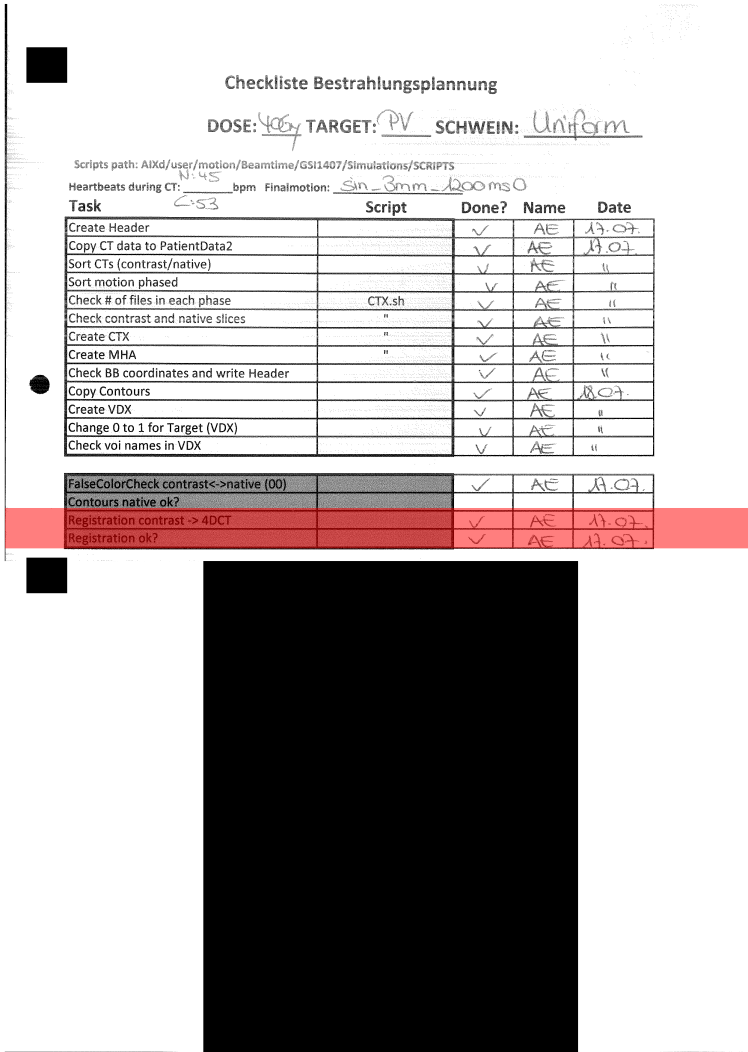
\includegraphics[width=0.8\textwidth]{./Vmm/Images/checkList.png}
		\caption{(a) A part of the checklist for quality assurance during the pig irradiation. DIR and DIRQA part is highlighted in red and consisted of two steps. First, DIR was made on a cardiac 4D-CT and afterwards DIRQA was made on
		DIR from state 50\%. The final result was presented as text shown in (b). The relative absolute difference stands for ratio between the true and default absolute difference.}
		\label{checkList}
	\end{center}
\end{figure}
\newpage
\begin{figure}[H]
	\begin{center}		
		\includegraphics[width=0.9\textwidth]{./Vmm/Images/AbsDiff_pigs.png}
		\caption{(a) Mean true and inverse absolute difference plotted against mean default absolute difference. The solid line shows a linear fit, with parameters
		written in the top left corner. Dashed line shows $y(x)=x$. (b) Box plots of mean default absolute difference distribution across nine 4D-CT states. Boxes represent 25-75\%, whiskers 10-90\%
		of data. The median is shown with a solid line, the mean is represented with squares and outliers with crosses.}
		\label{absDiff_pigs}
	\end{center}
\end{figure}

\subsubsection{Results}

An example of a pig cardiac 4D-CT DIR is shown in Fig.~\ref{exampleReg_pigs}. One DIRQA during the animal study showed higher mean true absolute difference than mean default absolute difference. The registration
was therefore repeated with three stages instead of 2. The third stage had 100 iterations with resolution size ``1, 1, 1`` and grid size ''10``. All other DIRQA checks were positive.

A post-experiment statistical analysis on vector field magnitudes is shown in Table~\ref{tab:vectordata_pig}. No statistical difference was
observed between the true and the inverse vector fields. However, significant differences were observed between the vector field magnitudes of PM and noPM groups. The contributions to vector field magnitudes from three axis were equal. 


\begin{table}[H]
  \centering
%   \footnotesize
  \caption{Data for vector magnitudes. Values are presented as mean (range).}
  \begin{tabular}{|c|c|c|c|c|}
  \hline\hline
	    & \multicolumn{2}{|c|}{PM} & \multicolumn{2}{|c|}{noPM} \\ \hline
  
            & True vector field   & Inverse vector field   & True vector field  & Inverse vector field \\
       \hline
	Mean & 0.08 (0.03 - 0.16) & 0.08 (0.03 - 0.14) & 0.07 (0.0 - 0.18)  & 0.06 (0.0 - 0.17) \\ 
	STD  & 0.4 (0.09 - 0.78)  & 0.36 (0.08 - 0.68) & 0.3 (0.05 - 0.77)  & 0.28 (0.04 - 0.71) \\ 
	Max  & 8.24 (1.6 - 17.33) & 7.98 (0.7 - 17.76) & 5.9 (0.97 - 15.91) & 5.38 (1.08 - 12.42) \\ 
    \hline\hline
  \end{tabular}
  \label{tab:vectordata_pig}
\end{table}

\begin{figure}[H]
	\begin{center}		
		\includegraphics[width=0.95\textwidth]{./Vmm/Images/exampleReg_pigs.png}
		\caption{An inverse color overlay of two states before (a) and after (b) DIR. The vector field is displayed on image (a) as arrows.}
		\label{exampleReg_pigs}
	\end{center}
\end{figure}

The dependence of the true and inverse absolute difference on default absolute difference with a linear fit is shown in Fig.~\ref{absDiff_pigs}a. 
The default absolute difference distribution across 9 states can be seen in Fig.~\ref{absDiff_pigs}b.

The distribution of the Jacobian and ICE results are shown in Fig.~\ref{jacobian_data_pigs}. Maximum values of true and inverse Jacobian and maximum ICE were
tested against maximum vector magnitudes and fitted with a linear function. Results are plotted in Fig.~\ref{maxvf_pigs}.

All linear fits in Fig.~\ref{absDiff_pigs} and ~\ref{maxvf_pigs} were statistically significant (p < 0.05).



\newpage

\begin{figure}[H]
	\begin{center}		
		\includegraphics[width=0.75\textwidth]{./Vmm/Images/Jacobian_data_pigs.png}
		\caption{Statistical data for true (top) and inverse (middle) Jacobian and ICE (bottom) for 9 cardiac 4D-CT states (reference state 0 is excluded) for 15 pigs. Mean, STD, maximum and minimum are represented as (a), (b), (c) and (d), respectively.
		Minimum ICE is 0 throughout all states and pigs. Boxes represent 25-75\%, whiskers 10-90\%
		of data. The median is shown with a solid line, the mean is represented with squares and outliers with crosses.}
		\label{jacobian_data_pigs}
	\end{center}
\end{figure}

\newpage

% \begin{figure}[H]
% 	\begin{center}		
% 		\includegraphics[width=0.9\textwidth]{./Vmm/Images/ICE_pigs.png}
% 		\caption{Statistical data for ICE for 9 4D-CT states (reference state 0 is excluded) for 15 pigs. Mean, STD, maximum are represented as (a), (b) and (c), respectively. 
% 		Boxes represent 25-75\%, whiskers 10-90\% of data, median is shown with a solid line, mean with squares and outliers with crosses.}
% 		\label{ice_pigs}
% 	\end{center}
% \end{figure}

% \begin{figure}[H]
% 	\begin{center}		
% 		\includegraphics[width=0.9\textwidth]{./Vmm/Images/JacSum2.png}
% 		\caption{(a) Plot of negative natural logarithm of minimum Jacobian versus natural logarithm of maximum Jacobian. Linear fit is displayed with solid line and it's parameters are given in the corner. PM and noPM are shown with red squares and green circles, respectively.}
% 		\label{calcJac_pigs}
% 	\end{center}
% \end{figure}

\begin{figure}[H]
	\begin{center}		
		\includegraphics[width=0.9\textwidth]{./Vmm/Images/MaxVfdata_pigs.png}
		\caption{Values of maximum Jacobian (a), minimum Jacobian (b) and maximum ICE (c) plotted against maximum vector magnitudes. A linear fit is displayed with a solid line and
		its parameters are written below the plots. The dashed line in (c) shows $y(x)= x$ plot. Values from cardiac 4D-CT state on image (d) are highlighted with blue squares in (a)-(c). PM and noPM are shown with red squares and green circles, respectively.
			ICE is displayed on (d) using the color table as displayed in the legend.}
		\label{maxvf_pigs}
	\end{center}
\end{figure}

\subsubsection{Discussion}

All 15 pig 4D-CTs have been registered, which resulted in 270 DIRs. DIRQA was performed in two steps - a smaller DIRQA during animal study on one state and a complete DIRQA on all 4D-CT states afterwards.

Mean vector field magnitudes were small (approx. 0.1 mm), since pigs were in a breath-hold position and the only motion was the heartbeat. 
Despite the small mean vector magnitudes it was still enough to observe statistical difference between PM and noPM.
Consequently, the difference between the two groups is consistent throughout the DIRQA.

DIR did well in terms of lowering the absolute difference. There was a strong correlation between default versus true and inverse absolute difference. 
The slope of the linear fit on Fig.~\ref{absDiff_pigs} has the same value than the slope from lung 4D-CT (see Fig.~\ref{absDiff_lung}), showing
the effectiveness of the B-Spline algorithm. The distribution of the default absolute difference across different states is smaller than in lung 4D-CT (10 HU compared to 35 HU), due to the fact
less motion was present in a pig cardiac 4D-CT. The shape of default absolute difference
distribution persist then in the Jacobian and ICE distributions as well. 

A good result in absolute difference does not necessary mean a good DIR, as can be seen from Jacobian and ICE checks. The mean Jacobian and ICE were 1 and 0, respectively, since the
vector fields were small on average. However there were large deviations present in Jacobian and ICE. Most notably, there were a few cases of negative minimum Jacobian which would suggest 
organ folding. Since organ folding does not occur during a heart beat, negative minimum Jacobian points to inconsistencies in DIR. 

The large deviations in Jacobian and ICE can in part be explained with large maximum vector field values, as shown in Fig.~\ref{maxvf_pigs}. All linear fits have a good correlation, with no
difference between PM and noPM in the quality of the fits. The actual linear fit parameters, however, further show the inconsistencies in DIR. The clearest example of inconsistencies in
DIR is with a linear fit from maximum ICE PM, which lies above the function $y(x)=x$. This means that there were points further away from the starting point after the true and inverse transformation, 
then just after true transformation. The linear fit for noPM maximum ICE showed better results in this terms, since it lied below the $y(x)=x$ function.


During the animal study only one DIR was repeated because of DIRQA. It was shown in post-experiment analysis, that most of the DIRs should be repeated, pointing out flaws in initial DIRQA procedure.
Mainly, DIRQA should be made on all DIR and not just on one state, since DIRQA from one DIR does not guarantee the quality of the other DIRs from the same 4D-CT. 
Each DIR is performed individually and should be treated as such. Furthermore, instead of mean Jacobian and ICE, maximum and minimum should be investigated, 
because it points to the worst part of the DIR.



% \subsection{Mid-Position patient example}


\section{Summary and Discussion}
\label{Summary}

Tools to perform DIR and DIRQA have been presented in this chapter. Modules were written for an open-source software Slicer that can handle large DIR problems, such as registering whole 4D-CTs. 
In addition to DIR, the modules can also provide quantitative information on DIR quality.
The main objective of this work was to provide a systematic approach for DIR and to give parameters on DIRQA that can estimate the quality of DIR. A first analysis of DIRQA checks was done on a large DIR database - 684 DIR were checked in total.

Most of the work was based on Slicer, which is a well-established software in medical research. To date, there are more than 500 publications that have used Slicer in their research \cite{SlicerCitation}, with topic ranging from 
teaching \cite{Pujol2016}, disease staging \cite{Liu2015, Liu2016b}, motion tracking \cite{Behringer2015} to image reconstruction \cite{Meyer2015}, image registration \cite{Li2015, Fedorov2015, Li2015b}
and others. Slicer offers ample functionalities and is especially suited for research, since it can be modified to specific needs. However, it is important to stress that Slicer 
is not a medical product and as such can not be used in clinic. Additionally, Slicer can sometimes be unstable with unexpected crashes. It is constantly under development and more and more errors
are fixed with each new release. New releases also bring new functionalities, but there can be problems with backtrack compatibility. 
% Even though there are some disadvantages to using Slicer, it's advantages
% outweigh them and make Slicer a useful tool, as was shown in this chapter.

Results shown in this chapter were obtained with the B-Spline DIR algorithm. Several other algorithms exist, demons most commonly used alongside B-Spline \cite{Thirion1998}. Varadhan et al. compared B-Spline and demons DIR
for lung cases \cite{Varadhan2013} and showed that B-Spline is superior to demons, especially if there is a difference in contrast between the images. They used a mutual information
metric, to account for differences in contrast. Images used in this chapter were either all without (lung 4D-CTs) or all with (animal study 4D-CTs) contrast agent, therefore no difference in contrast
between images was present and mutual metric could not be used.
% . Mutual information metric was tested as well for DIR. For lung 4D-CT it could not complete DIR, because the states are too similar, however for the results were worse than mean square error metric. For lung 4D-CTs 

A designated module was written for DIRQA. The main advantage of the DIRQA module is that all different techniques are gathered in a single place and can be used on a specific case. 
The ease of use is also essential, for DIRQA to find its way into clinical work flow.
A test of using DIRQA in potential clinical work flow was done at GSI during the animal study, where different users operated with both DIR and DIRQA modules. The experiment was carried out under time pressure, since there was
a scheduled beam time. 4D-CTs were acquired approximately two weeks before the scheduled irradiation. During this two weeks contour delineation, DIR, DIRQA, treatment planing 
and treatment planning QA had to be done \cite{Graeff2014a}.
There were already propositions for frameworks for DIRQA in clinical work flow \cite{Varadhan2013}, however none were tested in an actual clinical environment. An animal study can not be directly compared to an actual clinic,
however the number of pigs studied was high (15) and the study was under time constraint, which simulate some of the pressures present in clinical environment.

The techniques used in DIRQA were divided into visual qualitative (inverse color, checkerboard) and quantitative (absolute difference, Jacobian and ICE). While the quantitative can be used to pinpoint errors in DIR, the visual qualitative
can be used to actually locate the error as shown in Fig.~\ref{maxvf}d. The location and size of DIR error also determines if a repetition of DIR is necessary.
All three quantitative checks have been used in literature as a possible DIRQA \cite{Varadhan2013, Leow2007, Christensen2001, Bender2009}.
They all share the same flaw, however, that they are a necessary but not sufficient condition for a successful DIR. 
One common DIRQA check in literature that our module is currently missing, is comparison of anatomical correspondence - 
comparison between reference, moving and warped contours. Ideally the warped and the reference contour should be the same. Two metrics are usually used in contour comparison -
dice similarity coefficient \cite{Varadhan2013} and Hausdorff distance \cite{Huttenlocher1993}. Slicer already has functionalities for both contour comparison checks, so they could be used. 
The biggest disadvantage of the anatomical correspondence check is that the contour delineation is required in both, the reference and moving phase, which is scarcely done by physicians, 
since it takes too much time. Additionally, the anatomical correspondence check does not judge the vector field quality inside contour.
The lack of contours in both reference and moving phase was the reason the anatomical correspondence check was not used.

Studies on DIRQA so far have focused on a small number of DIR cases, whether it is phantom \cite{Mutic2001,Moore2004} or patient studies \cite{Wu2008, Varadhan2013}. With a small number of DIRs,
it is possible to thoroughly examine each DIR and hence understand DIRQA. In this work a different approach was
used. Rather than examining each DIR individually, a large dataset was analyzed and common traits for DIR were found. Due to differences in anatomical sites, 
DIRQA parameters have to be found for each anatomical site individually, since they can
deviate significantly, as seen by two different cases presented here. However, three checks are independent on anatomical site: mean true and absolute difference should be lower than 
default absolute difference, Jacobian should be positive and ICE should be smaller than maximum vector field magnitudes. 
If any of these checks fails, DIR needs to be investigated and, if necessary, repeated.
%However there may be parameters that persist throughout different anatomical sites, scaled Jacobian in particular.

DIR of a lung 4D-CT can be considered relatively easy, since the contrast between lungs and other tissue is high. 
This is confirmed by a mean value of 1 for the Jacobian and mean ICE smaller than 1 mm. The maximum and minimum Jacobian and ICE are more interesting, since they show 
DIR inconsistencies. All ICE values bigger than maximum vector field magnitudes were found to originate from areas with a poor DIR. An effect of a poor DIR can be seen in Fig.~\ref{contourPropagation},
where the propagated liver and lung contour do not match features on the image. An image artifact was the reason for the poor DIR. After investigation of poor DIR location and size, 
it was decided, that DIR does not require repetition, due to large distance between poor DIR and the tumor.
%This is supported by Fig.~\ref{calcJac_lung} and \ref{maxvf}. A small
%artifact was found in one phase and it was responsible for deviation from linear fit. Deviation from linear fit in Fig.~\ref{maxvf}a-c was also used to spot DIR inconsistencies
%and a lung image artifact was found in a different patient.

If the DIR of lung 4D-CT was considered relatively easy, opposite holds true for DIR of animal study 4D-CT. The motion of the heart during a heartbeat is complex, 
with muscles relaxing and contracting in different directions \cite{Seeley2007}. Furthermore,
the volume of blood shifts from one ventricle to the other. In the case of a cardiac 4D-CT, blood carried a contrast agent and blood distribution in heart was changing during a heartbeat. 
Therefore the HU distribution varied drastically in different cardiac 4D-CT states. Additionally, it is well established that pacemakers cause several complications in a CT scan \cite{Mak2012}. This was
confirmed by the differences observed between PM and noPM. The clearest example is the PM linear fit of the maximum ICE in Fig.~\ref{maxvf_pigs}, which is above $y(x) = x$. For noPM the linear
fit is below $y(x)=x$, however the slope has still a value of 0.77, compared to 0.38 of a lung 4D-CT fit. Inconsistencies in DIR were further supported by negative minimum Jacobian, which were found for both,
PM and noPM groups. Negative minimum Jacobian and large ICE values are clear indicators, that DIR in heart can not be 
accepted for heart treatment planning and needs to be repeated. An effect of DIR on actual irradiation also has to be examined.
The DIR of cardiac 4D-CT is currently under careful investigation
and several different solutions, such as artifact removal and different registration parameters are being tested.

In the future, the DIRQA module should undergo further testing. In addition to checking DIRQA on different anatomical sites and between different modalities, 
it should be investigated how good DIRQA is at spotting inconsistencies in DIR, i.e. what is the number of false negatives. Furthermore, with more
data analyzed, the parameters in DIRQA checks should get more precise, so outliers could be more easily spotted.

Based on the findings presented here, several new features could improve the DIRQA module. Instead of the mean, STD, maximum and minimum values, histograms could be displayed for quantitative tests.
Furthermore, histograms could be displayed for a specific contour, such as the tumor, which would give a direct indication of DIR quality effect on treatment planning. 
Additionally, the module should automatically show the location of maximum and minimum Jacobian and maximum ICE.
The worst part of DIR could be than immediately recognized and appropriate response could be formed.  

%   
%   \setcounter{mtc}{3}
%   \chapter{Comparison of Photons versus Carbon Ions in Single Fraction Therapy of Lung Cancer}
\label{PatStudy}


\section{Introduction}

Lung cancer is one of the leading medical problems worldwide with approximately 1.4 million deaths per year \cite{Siegel2014}. Surgery is usually the first choice in treating localized non-small cell lung cancer (NSCLC). However, in recent years stereotactic body-radiation therapy with photons (SBRT) showed very promising results, with high local control-rates of NSCLC \cite{Baumann2009, Fakiris2009, Grutters2010, Ricardi2010, Timmerman2010, Greco2011}.

Scanned particle therapy can produce sharp dose gradients with a finite range of the beam and can thus provide higher healthy tissue sparing. This reduces both side effects as well as the risk of secondary cancer \cite{Newhauser2011}. Treatment of lung tumors with particles is still challenging due to interplay and radiological path length changes \cite{Bert2011}.
The latter can be substantial when dense tissue (e.g. the solid tumor mass) is replaced with low-density tissue (lung) due to motion.

Grutters et al. have performed a meta-analysis on comparison between photon, proton and carbon ions in treating NSCLC \cite{Grutters2010}.
They found similar 5-year survival rates for SBRT, protons and carbon-ions (around 40\%). However, the number of patients treated with
particle therapy was low and they advise caution when interpreting the data. Also different fractionation schemes were used in the
comparison. A more recent review was published by  Kamada et al. \cite{Kamada2016} where they reported a high 3-year survival rate for
single-fraction carbon-ions (76.9\%), with no late treatment-related adverse effects. In comparison, SBRT had 55.8\% 3-year survival rate,
with 10 - 27\% of patients exhibiting grade 3 treatment-related adverse effects \cite{Timmerman2010}. It is important to note that all
of these studies used passive beam scattering, avoiding the problem of interplay between organ motion and scanning beam motion.
On the other hand, active beam scanning can provide even better dose shaping which becomes essential in high dose single fractionation
regimes. The effects of motion and motion mitigation techniques on scanned carbon ion dose distribution therefore need to be considered 
in a fair comparison of photons and carbon ions. 

To evaluate potential advantages of active scanning with carbon ions (PT), an in silico comparison of simulated PT plans to 
SBRT plans actually delivered was conducted. Target coverage and a wide range of OAR doses were assessed both with and without simulated motion on time-resolved computed tomographies (4D-CTs).



\section{Materials and methods}

\subsection{Patient data}

The study included 19 patients with in total 26 lesions that were actually treated with SBRT at the Champalimaud Centre for the Unknown, Lisbon (Portugal). The lesion size was 2.9 cm$^3$ (median, 25-75\% 1.4 - 9.7) and peak-to-peak motion was 3.1 mm (1.6 - 5.6). Three patients had two targets, one had five and the rest one. 13 lesions were right-sided, 12 were left-sided and one was located in right cardiophrenic space. An overview of tumor characteristics can be found in Table~\ref{tab:patdata}.
Two CTs were available for all patients. A planning CT was used for OAR delineation and SBRT planning. Target motion was estimated on a 4D-CT, consisting of 10 phases (0\% - 90\%). Clinical target volumes (CTV) were delineated using a registered positron emission tomography (PET) scan.

The planning objectives were that 99\% of planning target volume (PTV) must receive at least 24 Gy ($D_{99\%}$ $\geq$ 24 Gy) in a single fraction, while all OAR constraints as defined in the AAPM task group 101 report on stereotactic radiotherapy had to be respected \cite{Benedict2010}.

\newpage
\begin{table}[H]
  \centering
%   \footnotesize
  \caption{Lesion characteristics, with lesion locations, stages, peak-to-peak motions and volumes of corresponding CTV, PTV$_{SBRT}$ and PTV$_{PT}$. Abberevations for lesion location are: 
  RSL, right superior lung; IRL, inferior right lung; LSL, left superior lung; ILL, inferior left lung; RCS, right cardiophrenic space.}
  \begin{tabular}{|c|c|c|c|c|c|c|}
    \hline\hline
     & & & & \multicolumn{3}{|c|}{Volume (cm$^3$)} \\ \cline{5-7}
    \multirow{2}{*}{Number} & \multirow{2}{*}{Location} & \multirow{2}{*}{Stage} &
    Peak-to-peak & \multirow{2}{*}{CTV} & \multirow{2}{*}{PTV$_{SBRT}$} & \multirow{2}{*}{PTV$_{PT}$}\\
     &  & & motion [mm] & & & \\
    \hline
    1 & LSL & IIa & 4.8 & 35.9 & 100 & 179 \\
    2 & LSL & Ia & 3.1 & 1.6 & 7.7 & 40.6 \\
    3 & IRL & IV & 12 & 2.3 & 11.6 & 32 \\
    4 & RSL & Ia & 0.5 & 6.9 & 25.2 & 38 \\
    5 & ILL & IV & 4.4 & 2.5 & 15 & 20.5 \\
    6 & ILL & IV & 7.5 & 1.4 & 7.7 & 26.5 \\
    7 & RSL & IV & 3.9 & 16 & 40 & 72.5 \\
    8 & ILL & IV & 0.6 & 139 & 261 & 255 \\
    9 & LSL & IV & 2 & 9.2 & 35 & 46.5 \\
    10 & IRL & IV & 3.4 & 10.2 & 38 & 45.5 \\
    11 & ILL & IV & 2.8 & 14.4 & 46.4 & 57.2 \\
    12 & ILL & IV & 5.8 & 3.8 & 17.4 & 23.4 \\
    13 & RSL & IV & 0.8 & 4.3 & 17.7 & 26.3 \\
    14 & LSL & IV & 3.4 & 2.7 & 14.5 & 23.1 \\
    15 & RSL & IV & 2.1 & 3.1 & 15.4 & 33.5 \\
    16 & LSL & IV & 0.5 & 0.5 & 5.4 & 6.7 \\
    17 & ILL & IV & 7.8 & 0.8 & 6.1 & 23.5 \\
    18 & LSL & IV & 0.1 & 1.7 & 15 & 23.5 \\
    19 & IRL & IIIb & 11.4 & 27 & 137 & 118.5 \\
    20 & RSL & Ia & 2.2 & 1.7 & 10 & 23.4 \\
    21 & RSL & IV & 0.2 & 0.9 & 3.2 & 14.9 \\
    22 & RSL & IV & 2.2 & 3.9 & 22.1 & 27.5 \\
    23 & LSL & IV & 3.1 & 9.8 & 28 & 51 \\
    24 & RSL & IV & 8.1 & 0.6 & 3.3 & 4.1 \\
    25 & LSL & IV & 1.4 & 0.8 & 5.9 & 10 \\
    26 & RCS & IV & 11.8 & 0.4 & 6.6 & 8.6 \\

    \hline\hline
  \end{tabular}
  \label{tab:patdata}
\end{table}

\subsection{Planning target volume definition}

To account for range changes relevant for particles only, different PTV definitions were used for SBRT and PT, as shown in Fig.~\ref{Fig:PTV_def}. Within this chapter they will be named PTV$_{SBRT}$ and PTV$_{PT}$ for SBRT and PT, respectively.
In SBRT, the responsible clinician determined the maximum breathing motion of the CTV from the 4D-CT, hence creating an ITV. This ITV plus an additional 3 mm for setup uncertainty yielded the PTV$_{SBRT}$.

PTV$_{PT}$ was constructed following principles from Graeff et al \cite{Graeff2012}. Each beam has a unique PTV$_{PT}$. For setup uncertainty margins of 3 mm laterally and 1 mm in beam’s eyes view (BEV) were used on the CTV. Afterwards a water-equivalent path length ITV (WEPL-ITV) was build, using transformation maps from the B-Spline deformable registration of the 4D-CT data \cite{Shackleford2010}. Additional 2 mm + 2\% proximal and distal margins were added in BEV to account for uncertainty from Hounsfield units to water equivalent path length conversion.
If the target overlapped with an OAR (e.g. small airways) then OAR plus a margin of 2-5 mm was subtracted from PTV$_{SBRT}$ or PTV$_{PT}$.


\begin{figure}[H]
\begin{center}
\includegraphics[width=0.8\textwidth]{./PatientStudy/Images/Figure1.png}
\caption{Different PTV definitions for SDRT (PTV$_{SBRT}$) and CiT (PTV$_{PT}$). For PTV$_{SBRT}$ isotropic margins of 3 mm plus maximum tumor displacement due to 
breathing were used on the CTV; For PTV$_{PT}$ margins of 3 mm laterally and 1 mm in beam’s eye view were used and then range-ITV was constructed with
2 mm + 2\% range margins added for PTV$_{PT}$ in end-inhale phase.}
\label{Fig:PTV_def}
\end{center}
\end{figure}

\newpage

\subsection{SDRT treatment planning}
\label{SBRTTP}

The clinical plans were calculated with the Eclipse v10 planning system (Varian Medical Systems, Palo Alto, USA) using the AAA beam model. They were all VMAT plans generally consisting of 4 overlapping partial arcs, 2 in clockwise and 2 anticlockwise direction, with a gantry range of typically 200°. For tumor sizes > 2.5 cm a calculation grid of 2.5 mm was used, otherwise this was 1 mm. During optimization, a first iteration included the PTV$_{SBRT}$ only, after which the OARs were added. In order to lower OAR dose and improve the PTV$_{SBRT}$ homogeneity, we created an artificial shell of 2 cm around the PTV$_{SBRT}$ and minimized the dose there as well. During optimization the fast Multi Resolution Dose Calculation (MRDC) model was used, with one intermediate step using the slower but more accurate AAA model to get an adequate PTV$_{SBRT}$ coverage after optimization.


\subsection{Carbon-ions treatment planning}
\label{PTTP}

For PT, state of the art 4D treatment planning software TRiP98 was used \cite{Richter2013}. A single field uniform dose plan (SFUD) 
was optimized on the PTV$_{PT}$ in the end-inhale reference phase of the 4D-CT. Most targets ($n=20$) were planned with two fields. 
For the remaining targets, one ($n=1$), three ($n=3$) or four ($n=2$) fields were used due to proximity of OARs. 
A regular grid of beam spots with a spacing of 2 mm, a beam spot full width at half maximum (FWHM) size of approximately 6 mm and a 
3 mm ripple filter were used. To compensate for short particle ranges in lung tissue, a bolus of 80 mm water-equivalent thickness 
was added.

The relative biological effectiveness (RBE) following the local effect model (LEM) IV \cite{Elsaesser2010}. 
For a conservative estimation, an alpha-beta ratio of 6 Gy and 2 Gy were used for target and OARs, respectively. 
This led to an RBE of approximately 1.1 in target tissue and approximately 1.1 to 3 in OARs.
Dose was calculated on end-inhale (3D-Dose$_{0\%}$) and end-exhale (3D-Dose$_{50\%}$) phases. 
4D dose delivery was simulated as described by Richter et al \cite{Richter2014}. Two different breathing periods (3.6 and 5 s) 
and two different starting phases (0° and 90°) were used. Simulations without motion compensation (4D-Dose$_{interplay}$)
and with slice-by-slice raster rescanning were performed (4D-Dose$_{rescan}$). Five rescans were used for the majority 
of targets (n=24), whereas 20 rescans were used for targets where the interplay effects were too big to achieve a 
satisfactory target coverage ($n=2$; lesions 3 and 18 in Table~\ref{tab:patdata}). 


%\begin{figure}[H]
%\begin{center}
%\includegraphics[width=0.9\textwidth]{./PatientStudy/Images/RBE.png}
%\caption{RBE distribution in a patient (a) depends on a actual dose profile (b).}
%\label{Fig:RBE}
%\end{center}
%\end{figure}

\subsection{Dose metrics and analysis}

For comparison between SBRT and PT the following dose metrics were used - for the target the minimum dose in 99\% of the volume ($D_{99\%}$), which should be higher than 24 Gy; for OARs, the maximum point dose ($D_{Max}$) and the mean dose ($D_{Mean}$). Additionally, the volume receiving 20\% of the planned dose ($V_{20\%}$) was used to assess differences in lung doses. In all cases, absorbed dose in Gy for SBRT was compared to biologically-equivalent dose in Gy(RBE) for PT.

Paired t-tests were performed to compare the dose metrics and for post-hoc exploratory analysis between groups a two-sided t-test with Welch correction for different variances was carried out. A p-value < 0.05 was considered significant. Dose differences are always reported such that higher dose levels for SBRT result in positive values.



\section{Results}

Examples of two SBRT and 4D-Dose$_{rescan}$ PT treatment plans are shown in Fig.~\ref{Fig:TreatmentPlans}. Patient 9 has two lesions in close proximity to the spinal cord. Patient 2 has a small lesion (1.6 cm$^{3}$) in the superior position of the left lung. $D_{99\%}$ is 100\% for SBRT and PT in all CTVs for Patient A and B; average OAR difference between SBRT and PT in $D_{Max}$ is 5.1 Gy and 1.4 Gy and in mean dose 1.4 Gy and 0.7 Gy, respectively for patient A and B.


\begin{figure}[H]
\begin{center}
\includegraphics[width=0.9\textwidth]{./PatientStudy/Images/Figure2.png}
\caption{Treatment plans for SBRT (left), PT (middle) and dose volume histogram (right) for SBRT (solid lines) and PT (dashed lines) for two patients. PT curves for OARs without any dose are not shown. Patient 9 (top row) might be better suited for PT and patient 2 (lower row) for SBRT. Patient 2 has a small lesion (1.6 cm$^{3}$) in a central lung region, resulting in large PTV$_{PT}$ - up to 32 cm$^{3}$, compared to PTV$_{SBRT}$ 7.7 cm$^{3}$. The CTV contour is outlined in white.}
\label{Fig:TreatmentPlans}
\end{center}
\end{figure}

\subsection{Target Coverage}

Difference in PTV definition resulted in 1.5 (1.3 - 2.1) times bigger PTV$_{PT}$ than PTV$_{SBRT}$. All SBRT plans were clinically acceptable, though in one case the $D_{99\%}$ was reduced to 16.8 Gy due to proximity of an OAR. 3D-Dose$_{0\%}$ and 3D-Dose$_{50\%}$plans provided sufficient target coverage in all patients. For 4D-Dose$_{interplay}$ and 4D-Dose$_{rescan}$ there was 63\% and 2\% cases of insufficient target coverage, respectively, across all targets and different breathing patterns. Details are shown in Fig.~\ref{Fig:InterplayDiff}. For the patient with reduced dose in SBRT, PT could increase the $D_{99\%}$ from 16.8 Gy in SBRT to 20.3 Gy while adhering to OAR constraints. 


\begin{figure}[H]
\begin{center}
\includegraphics[width=0.9\textwidth]{./PatientStudy/Images/Figure3.png}
\caption{CTV $D_{99\%}$ for SBRT and different PT calculations. Four different breathing patterns are included for all targets in 4D-interplay and 4D-rescan. The dashed line shows the lower limit for clinical acceptance. One patient was an exception where lower target dose was accepted due to the proximity of a critical structure.  }
\label{Fig:InterplayDiff}
\end{center}
\end{figure}
\newpage
\subsection{Dose in OARs}


There was no significant difference in dose to OAR between the different PT dose calculations. 
The $D_{Max}$ and $D_{Mean}$ for SBRT and 4D-Dose$_{rescan}$ for OARs heart, spinal cord, smaller airway esophagus, trachea, aorta, ipsi- and contralateral lung are 
presented in Table~\ref{tab:results}.There was a significant difference in both $D_{Max}$ and $D_{Mean}$ for all OARs between SBRT and PT, with 
PT delivering less dose to OARs. Significant difference was also observed for $V_{20\%}$ for ipsilateral lung, which was 15.3\% (9.6 - 23.5) and 10.3\% (7.9 - 13.7) for SBRT and PT, 
respectively. The $V_{20\%}$ for contralateral lung was zero for almost all patients in SBRT and PT. The overall OAR difference for patients between SBRT and PT 
was significant, 2.8 Gy (1.6 - 3.7)  for $D_{Max}$ and 0.7 Gy (0.3 - 1.6) for $D_{Mean}$. 



\begin{table}[H]
  \centering
%   \footnotesize
  \caption{Dose metrics for OARs. First value at each organ is from SDRT and the second from 4D-rescan. All values are shown as median and 25-75\% in brackets.}
  \begin{tabular}{l|c|c|c|c|}
    \cline{2-5}
     & \multicolumn{2}{|c|}{$D_{Max}$ (Gy)} & \multicolumn{2}{|c|}{$D_{Mean}$ (Gy)} \\
     \hline
    \multicolumn{1}{|l|}{OAR} & Photon & Carbon & Photon & Carbon	\\
    \hline
\multicolumn{1}{|l|}{Heart} & 6.0 (0.3 - 11.6) & 0 (0 - 8.8)	& 1.3 (0.1 - 2.2) & 	0 (0 - 0.5) \\
\multicolumn{1}{|l|}{Spinal Cord} &	5.5 (3.3 - 8.5)	& 0 (0 - 0.5) &	0.7 (0.3 - 1.2) &	0 (0 - 0) \\
\multicolumn{1}{|l|}{Smaller Airways} & 13.0 (9.8 - 17.1) &	10.3 (3.3 - 19.1) &	2.8 (1.5 - 5.8) &	0.5 (0 - 2.6) \\
\multicolumn{1}{|l|}{Esophagus} & 5.8 (3.9 - 8.4) &	0 (0 - 0.3) &	1.1 (0.6 - 1.5) &	0 (0 - 0)\\
\multicolumn{1}{|l|}{Trachea} &3.9 (1.8 - 5.4) &	0 (0 - 0) &	1 (0.3 - 1.3) &	0 (0 - 0)\\
\multicolumn{1}{|l|}{Aorta} & 8.0 (5.1 - 21.9) &	3.9 (0 - 18.1) &	1.4 (0.7 - 1.6) &	0.1 (0 - 0.4)\\
\multicolumn{1}{|l|}{Ipsilateral Lung} & 26.3 (26.0 - 26.5) &	26.3 (25.8 - 26.5) &	1.9 (1.5 - 3.0) &	1.9 (1.4 - 2.5)\\
\multicolumn{1}{|l|}{Contralateral Lung} & 5.0 (3.5 - 9.6) &	0 (0 - 0.9) &	0.4 (0.2 - 0.6) &	0 (0 - 0) \\
    \hline\hline
  \end{tabular}
  \label{tab:results}
\end{table}




\subsection{Dependence on CTV Size}

Significant differences were observed between patients with a single CTV smaller ($n=8$) or larger ($n=7$) than 2.5 cm$^{3}$ for $D_{Max}$ and $D_{Mean}$, see Fig.~\ref{Fig:OAR_boxplots}. For patients with a smaller CTV, the dosimetric advantage over SBRT was on average 0.9 Gy and 0.5 Gy lower for $D_{Max}$ and $D_{Mean}$, respectively. This was associated with PTV$_{PT}$ definition - the average volume ratio between PTV$_{PT}$ and PTV$_{SBRT}$ was 2.9 (1.6 - 4.0) and 1.5 (1.3 - 1.8), for patients with CTV < 2.5 cm$^{3}$ and CTV > 2.5 cm$^{3}$, respectively.

The 4 patients with multiple lesions were excluded from this comparison. The $D_{Max}$ and $D_{Mean}$ difference were on average higher in these patients, but the number of patients was too low for statistical analysis. 


\begin{figure}[H]
\begin{center}
\includegraphics[width=0.9\textwidth]{./PatientStudy/Images/Figure4.png}
\caption{Box plots of average OARs max point dose ($D_{Max}$) and mean dose difference between SBRT and PT for patients with single CTV smaller ($n = 9$) or bigger ($n = 6$) than 2.5 cm$^{3}$. Boxes represent 25\% - 75\%, outliers are shown as whiskers and median is shown with solid lines. Values for patients with multiple lesions are shown with circle symbols.}
\label{Fig:OAR_boxplots}
\end{center}
\end{figure}


\section{Discussion}

This is the first in silico trial directly comparing clinically valid SBRT plans to scanned carbon ion plans using state of the art 
4D dose calculation and motion mitigation methods for NSCLC patients. Our study found that PT deposited less dose to OARs compared 
to SBRT. Therefore PT might be considered as an alternative treatment option to SBRT. The finite range of the beam permits a small 
number of fields and thus a narrow entry channel, so that critical OARs such as spinal cord, heart, esophagus, and the contralateral 
lung could be effectively spared using PT, with typically low or even zero dose. PT could be thus highly beneficial to patients with 
impaired contralateral lung function, because PT deposited no dose in the contralateral lung in 12 patients, while SBRT irradiated 
the contralateral lung in all patients. Being an intensity-modulated arc therapy, SBRT had an advantage in some patients where the 
smaller airways were in a close proximity to CTV; SBRT could shape the dose distribution to reduce dose to the smaller airways, 
compensating PT's advantageous physical dose characteristics.

Further increase in OAR sparing could be achieved by using intensity modulated particle therapy (IMPT) instead of SFUD. 
While IMPT could lead to less dose in the OARs, it would make the plans less robust against setup errors due to 
additional dose gradients between the fields. These gradients can be controlled by employing robust optimization to 
account for range, motion and setup uncertainties, which we will implement in a future 4D treatment 
planning study \cite{Chen2012, Graeff2014}.



\subsection{Range Margins and Motion Mitigation}

Since conventional geometric margins are not suitable for PT \cite{Park2012}, margins based on range changes were used. Another trial comparing photon to proton therapy in NSCLC patients also used different PTV definitions to incorporate 
range changes \cite{Roelofs2012}. As shown in our study, inclusion of range changes leads to increase in PTV$_{PT}$, up to 4.7 times compared to PTV$_{SBRT}$. 
Furthermore, the difference between PTVs is bigger for smaller tumor sizes. Patients with bigger tumor volumes (CTV > 2.5 cm$^{3}$) are therefore better suited for treatment with PT. 

Our results confirm previously published results that interplay can lead to a dose degradation in treating moving targets with active scanned beam \cite{Bert2008}. 
Figure 3 shows the importance of using 4D dose calculation and motion mitigation techniques in treating moving targets with particles. 
Even small motion amplitude can lead to underdosage in CTV without proper motion mitigation. Considering the average over the 4 simulated motion patterns, 15 patients showed a $D_{99\%}$ < 24 Gy under interplay 
conditions, as opposed to none when using rescanning (excluding the one patient with reduced target dose). Rescanning proved to be a strong mitigation technique, with robust results across all targets and different breathing patterns.

Recent studies suggest that some patients require phase-controlled layer or volumetric rescanning for sufficiently robust target coverage \cite{Mori2013,Takahashi2014}. 
The advantage of simple slice-by-slice rescanning is that no motion monitoring or assumptions on the breathing frequency are necessary \cite{Bert2011}, but the higher required number of rescans 
might increase treatment times due to reduced beam intensities. Another possibility is to combine rescanning with gating, which was already sucm$^{3}$essfully implemented in clinic \cite{Rossi2016}.




\subsection{RBE and Proton Therapy}

Carbon ions exhibit a radiobiological advantage, especially in the Bragg peak region. However, for high doses as used here the effect of RBE is not well documented and is subject to ongoing research \cite{Friedrich2014}. 
For these high doses RBE for carbon ions should approach a value between 1 and 2 \cite{Carabe2007}, which is in agreement with values in our study (around 1.1).

Coincidently, RBE values in the target at high doses are similar to those used clinically in proton therapy. Carbon-ions show considerably lower lateral scattering though, which should result in even better 
OAR sparing than protons. Our results are in agreement with several in silico studies comparing SBRT and proton therapy for NSCLC \cite{Roelofs2012, Kadoya2010, Register2010}. 
Furthermore, a study made by Kadoya reached the same conclusion as our study, that patients with larger CTV and/or multiple CTVs would  receive less dose from proton therapy \cite{Kadoya2010}.
A recent phase II trial for patients with multiple sites of extracranial disease showed good results for photons \cite{Iyengar2014}, however, based on the findings of Kadoya et al and our study, 
proton and/or carbon-ion therapy might result in even better outcome. 



\subsection{Study limitations}


The 4D dose calculations were based on a regular breathing pattern, which typically varies during patient treatment and/or between 4D-CT acquisition and actual treatment \cite{Verma2010, Malinowski2011}. 
A possible solution was proposed by Boye et al. to get motion information from 4D magnetic resonance imaging (4DMRI) and use it in 4D dose calculations \cite{Boye2013}.

Furthermore, SBRT treatment plans were done on a static case in contrast to a 4D dose calculation done for PT. This should not influence the results of our study, 
since motion has a smaller impact on photon dose distributions \cite{Zou2014}, whereas it is imperative in PT dose calculations \cite{Bert2011}. 

There were also differences in treatment planning. PT plans were done by a single person in a research setting, whereas SBRT plans were made by different people under clinical conditions with the requirement to finish the plans on time. 

Slight changes also existed between the planning CT, used for SBRT treatment plans and 4D-CT used for PT treatment plans, even though 4D-CT was usually acquired right after the planning CT. 
The propagation of contours from the planning CT to the 4D-CT and also for the 4D dose calculation rely on deformable image registration (DIR), where even small changes can effect 4D dose distribution \cite{Kashani2008}. 
Results from DIR were thoroughly checked and results were presented in Chapter~\ref{chapter:vmm}. However, the transformation of the dose with DIR is a debated topic and might jeopardize the simulated results, especially with respect to the 4D target coverage. On the other hand, dose differences 
in OARs were large and should be robust against vector field errors in the order a few mm. Nevertheless, further studies are warranted, possibly using advanced moving phantoms for an experimental 
validation \cite{Perrin2014} and finally also clinical trials. First patients are being treated in thoracic and abdominal regions with an active beam scanning at the National Institute for Radiological Sciences (NIRS) in Japan \cite{Mori2016}.



\subsection{Application}

Scanned carbon ion therapy is available only in a limited number of clinics, mainly due to the considerably higher cost in comparison to photon linacs.
Therefore a careful patient selection appears sensible. Patients with larger and multiple lesions where SDRT might be limited due to OAR constraints 
could be referred to carbon centers. In this study, already lesions larger than 2.5 cm$^3$ were found to benefit significantly stronger from CiT.

\section{Conclusion}
SBRT and PT both achieved satisfactory target dose. In most patients PT deposited less dose in all OARs (including heart, spinal cord, esophagus, trachea and aorta). Patients with multiple lesions and/or with large target volumes might be preferentially selected for particle therapy.

%   
%   \setcounter{mtc}{4}
%   \include{ComplexPatients/ComplexPatients_main}
%   
%   \setcounter{mtc}{5}
%   \chapter{Discussion}

This is a first in silico study directly comparing clinical stereotactic body radiation therapy (SBRT) with scanned carbon-ions (PT) for non-small cell lung cancer (NSCLC). 
Our results show that PT could be considered an alternative to SBRT, with the same tumor coverage and less dose to OARs. Furthermore, the study was expanded to patients with multiple
NSCLC disease sites. With a state of the art 4D optimization, intensity modulated particle therapy (IMPT) was able to generate treatment plans with less OAR dose and comparable target coverage
to SBRT. It was possible to plan for a a single fraction ablative dose with IMPT for a specific patient, where SBRT was limited due to excessive heart dose.

Treatment of NSCLC with PT is influenced by interplay between tumor motion and beam scanning. It was shown that rescanning offers
adequate motion mitigation. 

PT offers precise dose shaping but it can thus also be more prone to uncertainties. Calculation of time-resolved (4D) doses can be significantly
affected by errors in deformable image registration - DIR \cite{Heath2006}. Special tools were developed in the scope of this thesis to ensure DIR quality assurance (DIRQA).
Tools were tested on a large dataset to ensure their validity.


\section{Deformable image registration and validation}

A single DIR algorithm was used in this study, B-Spline. In contrast to Demons algorithm, B-Spline should handle large deformations well as present in lung and cardiac 4D-CT \cite{Tang2013}.
The DIR for lung 4D-CT had only small inconsistencies and here B-Spline can be considered sufficient. On the other hand, the results suggest that B-Spline is inadequate for
DIR of a pig cardiac 4D-CT. The parameters used
in B-Spline DIR were similar in both cases of DIR. This could be improved by systematically investigating the effect of parameters on DIR quality. 

The advantage of using open-source software for DIR, as explained in Section~\ref{RegistrationImplement} is that different DIR algorithms, 
optimization metrics and image types can be used. They can be accessed either using
existing libraries, such as ITK \cite{Yoo2002}, or by writing designated software \cite{Fedorov2015}. In the future, different DIR algorithms have to be implemented 
and tested for various anatomical sites.

In this study, DIR was used in contour propagation and 4D dose calculation. The 4D dose calculation requires 
accurate DIR in each voxel, since dose is propagated with vector field. This was ensured by calculating vector field Jacobian and ICE voxel-wise. 
% An indirect conformation of DIR quality, or specifically small inverse consistency error (ICE) in target was flat target dose in 4D dose calculation. Target was propagated
% in different 4D-CT states using inverse DIR. The propagated states were used to create ITV on which the 3D dose was optimized. The 4D dose calculation is based on propagating dose
% from 4D-CT states to reference one with true DIR. If there were large inco
% Contours are propagated 
% with inverse registration

Tests in DIRQA module were divided into two groups - qualitative and quantitative. Qualitative tests are false color and checkerboard; they provide an overview of the DIR result.
However they do not give any information of vector field quality and it is impossible to review the sheer amount of data. An example of the disadvantage of the qualitative test could be seen in pig cardiac 4D-CT, where qualitative test did not show
any errors in DIR, but errors were observed in vector fields. 

The quantitative tests used in the DIRQA module are landmark distance, absolute difference, Jacobian and ICE. Absolute difference, Jacobian and ICE have undergone an extensive testing. The results suggest
that absolute difference gives us the least information about DIRQA, apart that it has to be lower after the DIR. 
We have shown that bigger deformations yield more deviations in Jacobian and ICE, which was also previously reported \cite{Stanley2013}. 
Furthermore, we have confirmed that Jacobian should always be positive for a successful DIR \cite{Rey2002}. Additionally, our results show that ICE should 
be smaller than maximum vector field magnitudes. Any deviations from mentioned trends should be thoroughly examined.

There are additional vector fields validation methods beside Jacobian and ICE, such as vector field curl \cite{Schreibmann2012}, unbalanced energy \cite{Zhong2007}, 
permutation, and analysis of variance (ANOVA) tests \cite{Klein2009}.
It was demonstrated in a study by Salguero et al. \cite{Salguero2011} that DIR errors greater than 1 mm can lead to large dose errors in high-dose gradient regions. 
Therefore the DIR accuracy has to be quantified at each image voxel in the high-dose 
gradient regions. In our study, a focus was given on a complete registration to find potential errors. However, in future studies the regions of interest used
should be around the target, where high-dose gradients can occur. Furthermore, the effect of image and vector field downsampling on DIRQA and on 4D dose calculation should be assessed.

%A solution to evaluate at each specific voxel and for patient-specific registration was given by Stanley at al \cite{Stanley2013}. 
%They proposed a computational phantoms and their deformations with a finite element module framework. 

Due to the lack of landmarks in all 4D-CTs, landmark distance was not included in the verification. Two contour based validations, dice similarity coefficient \cite{Varadhan2013} and Hausdorff distance \cite{Huttenlocher1993}
are planned to be implemented in the DIRQA module. In the literature many approaches have been reported to assess DIRQA with landmarks or contours. 
A study by Hardcastle et al. \cite{Hardcastle2012} 
compared demons and Salient-Feature-Based registration with dice coefficients between propagated and physician drawn contours.
A multi-institutional study by Brock et al. \cite{Brock2010} compared differences in propagated and oncologist drawn landmarks. 
A method has been developed by Castillo et al. \cite{Castillo2009} to automatically identify landmark points
in lung patients images. However, visual based evaluations are of limited use in regions of uniform image intensity and by the number of the objects being tracked \cite{Kashani2008, Liu2012}.



\newpage
\section{Treating non-small cell lung cancer with particle therapy}

The results in this thesis suggest that PT could be used as a treatment modality for NSCLC. It delivers comparable target dose to SBRT, while significantly reducing 
dose to OARs. The lower mean heart could be crucial in improving patient survival based on a recent trial from RTOG 0617 \cite{Bradley2015}. 
The mean dose to heart would be on average 1 Gy smaller with PT than with SBRT. 
For patients with multiple disease sites, it would be on average 4 Gy smaller, reaching up to 9 Gy. Similar results were observed when comparing protons to SBRT \cite{Georg2008}. 

The advantageous dose profile of PT permits to use few, selected fields with narrow entry channels, avoiding the dose bath needed in SBRT
to achieve high dose gradients in the target.
Hence the benefit of PT is most profound for patients with large total target volume, whether a large single target or multiple targets. Studies suggest, that SBRT is limited for large
tumors (radius > 5 cm) and multiple primary tumors \cite{Timmerman2006, Georg2008, Westover2012}, making PT a promising alternative.

Besides large tumors and multiple primary tumors, SBRT is also limited in treating centrally located tumors and tumors close to the chest wall.
In a study done at Francis H. Burr Proton Therapy Center 
patients who could not be treated with SBRT, due to the scenarios mentioned, were treated with passive proton beam in 3 - 5 fractions, 
delivering 42 - 50 Gy \cite{Westover2012}. They observed similar tumor local control rates as in SBRT (100\% in a two year follow-up) with limited toxicities. 
It should be stressed that these patients were rejected from SBRT treatment due to the complexity and regardless proton therapy achieved similar results
to SBRT.

In addition to the narrow entry channel, PT has sharper dose gradients and can conform the dose better to the target. Fig~\ref{Fig:InterplayDiff} shows that 80\% of the targets have $D_{99\%}$
between 100 - 107\% and 100 and 102\% for SBRT and PT, respectively. Sharper dose gradients also enable less dose to the surrounding tissue. Nevertheless, fraction escalation
was possible only in one patient out of three. The limitation in the two patients with unsuccessful fraction escalation was the esophagus maximum single point dose $D_{Max}$, 
which is 15 Gy in 1 x 24 Gy scheme. In both patients the esophagus was closer than 2 mm to the target, making the limitation impossible to respect without sacrificing target dose.
Furthermore, for one of these two patients, PT could not deliver planned target dose, whereas SBRT could. Beside complex geometry, the tumor had a small volume and 
large motion. This patient exhibits the advantage of SBRT over PT.

PT has to take into account particle range uncertainty, which can come from the conversion of HU to stopping power \cite{Schneider1996}
or from anatomical changes in the patient \cite{Unkelbach2009}. We included range uncertainties with expansion of target in beam's eye view, which resulted on average in 1.5 times bigger
target volume for PT compared to SBRT. Another way to include range and other uncertainties is robust optimization, resulting in IMPT plans more resilient to uncertainties \cite{Unkelbach2009, Chen2012}.
We are planning to include robust optimization in a future study, where SFUD, IMPT and robust IMPT plans will be compared for NSCLC patients.

While tumor motion influences photon treatment, it can be mitigated with proper margins \cite{Zou2014}. 
On the other hand, effects can be substantial when treating moving targets with scanned particle therapy \cite{Bert2008}.
It was shown in this thesis that rescanning is an adequate motion mitigation technique. However, rescanning has a degree of uncertainty, 
especially regarding OAR $D_{Max}$.
In hypofractionated treatment these limits are strict and exact dose to the OAR must be known. 
A possible solution would be to simulate rescanning and 4D delivery in the optimization process itself. 
Such a solution is not yet feasible due to the complexity of the problem. Another solution could also be phase-controlled rescanning with greatly reduced
uncertainty in the mitigation outcome \cite{Mori2013,Takahashi2014}. However,
it requires motion monitoring and complicates treatment delivery.

% The PT treatment planning for patients with complex geometry has to include 4D optimization and dose calculation as shown within this thesis. 
% A special consideration has to be taken in dose to OAR limits, since they can be breached under different motion patterens.
% Beam tracking \cite{Bert2007} or jet-ventilation \cite{Santiago2013} would be possible solutions, however, the former is not yet clinically avaliable and the latter 
% significantly complicates treatment.

Gating is a commonly used motion mitigation technique in both photon and particle treatment. While it provides less motion-induced dose errors, it prolongs treatment time.
A recent study by Zhang et al. \cite{Zhang2015} included 
different breathing patterns, obtained from MRI, on a 4D-CT and calculated 4D doses for liver cancer patients treated with proton therapy. They have shown that a gating window of 3 mm can result
in a 10\% efficiency of a duty-cycle, 
substantially prolonging treatment. Additionally, they have shown that neither volumetric or slice-by-slice rescanning could achieve good target coverage.
However, this was obtained with combination
of gating and rescanning. Their results suggest that a combination of gating and rescanning would currently be the best solution for treating NSCLC patients with PT.

Between rescanning, gating and beam tracking beam tracking is the most precise technique, since it requires no internal target margins \cite{Bert2011}. 
Current clinical implementations of tracking in photon radiotherapy \cite{Kilby2010, Keall2014} can not be directly used in particle therapy, 
since they only provide the position of single internal points. Fassi et al. 
\cite{Fassi2015} were able to account for inter- and intra-fractional variability of patient's anatomical configuration with a designated modeling technique \cite{Fassi2014}.
The measured median of water-equivalent path length in target was within 2 mm of a simulated one. For actual clinical implementation it will be necessary to test the model
on a large patient dataset.

All three techniques, rescanning, gating and beam tracking, essentially adapt 3D treatment plan to a 4D situation and thus have limitations. Full 4D-optimization, on the other hand,
creates a 4D treatment plan, with each motion state in the 4D-CT having a designated treatment plan. A full 4D-optimization has been successfully implemented and verified experimentally at
GSI \cite{Graeff2013}.

% Surgery is the gold standard for treating NSCLC in the early stages \cite{Roesch2014}. 
% In recent years, however, SBRT showed similar results as surgery and SBRT is recommended for all high-risk surgical patients. 
% A recent comparison study by Yu et al. \cite{Yu2015} showed that
% SBRT compared to surgery had lower intermediate mortality and toxicity. However, patients with long life expectancies were found to benefit more from surgery. 



% Treatment for early stage NSCLC is well established, however, more than 75\% NSCLC cases present themselves in an advanced stage \cite{Jemal2009}, 
% usually due to the lack of detection in the early stages. The standard of care for advanced NSCLC is concurrent chemotherapy \cite{Oshiro2014}.
% Dose escalation studies showed favorable prognosis for doses higher than 70 Gy \cite{Hayman2001, Rosenman2002, Socinski2008}. 
% The results of a recent phase 3 randomized trial by Bradley et al. \cite{Bradley2015}, however, showed better survival rates for patients administered 60 Gy,
% instead of 74 Gy. It was speculated that higher doses to heart and esophagus might have contributed to higher mortality rates \cite{Cox2012}. 
% Results presented in this thesis show that mean dose to heart and esophagus would be on average 1 Gy
% smaller with PT than with SBRT. For patients with multiple disease sites the the average mean heart and esophagus dose would be 4 and 3 Gy smaller.

In a recent phase II study by Iyengar et al. \cite{Iyengar2014} patients with stage IV NSCLC were treated with SBRT and chemotherapy. 
They have irradiated 52 targets in 24 patients, 16 of them had more than one target. The results were promising, with 20 months median overall survival, 
compared to 9 months when treating with chemotherapy only \cite{Tsao2008}. Results in this thesis show that patients with multiple disease sites 
would especially benefit from PT. Based on the poor prognosis of stage IV NSCLC patients and on the results published by Iyengar et al.,
stage IV NSCLC patients could be eligible candidates for PT treatment. Additionally, such patients usually exhibit chronic obstructive pulmonary disease and 
less dose to the lung is warranted \cite{Westover2012}. This further supports our claim, since our study showed substantial differences in 
doses to ipsilateral lung ($V_{20\%}$ was on average 15\% smaller in PT for patients with multiple disease sites) and 
contralateral lung as well - 70\% of patients did not receive any dose to the contralateral lung, whereas SBRT deposited dose in contralateral lung in all patients.

The results of a multi-institutional randomized trial, RTOG1308 \cite{RTOG1308}, comparing photons and particle therapy in treating NSCLC,
will have an important impact on treating NSCLC. The trial started in 2014.


\subsection{Outlook}

Recent advances in photon radiotherapy allow the use of non-coplanar beams, a so-called 4$\pi$ optimization \cite{Dong2013}. A study by Dong et al. \cite{Dong2013b} showed that
4$\pi$ yielded better target coverage and OAR sparing than SBRT for NSCLC patients. 
They have reported reduction of $D_{Max}$ in heart, esophagus and spinal cord by 32\%, 72\% and 53\%, respectively, showing
the potential of a 4$\pi$ optimization. According to this thesis, PT is able to reduce the $D_{Max}$ even further, with a reduction of 57\%, 87\% and 83\% for heart, esophagus and spinal cord,
respectively. The numbers, however, should be compared with caution, since they were obtained from a different set of patients. 
A future study, directly comparing SBRT, $4\pi$ and PT for NSCLC is thus warranted.

Robust optimization seems to be gaining on popularity for PT. Standard margin definition to account for uncertainties fails in PT, while the inclusion of uncertainties in 
optimization process can substantially improve treatment plans \cite{Chen2012}. The robustness optimization is now computationally possible even for a 4D optimization \cite{Liu2016}, opening a wide
field of new possibilities. 
\newpage

\chapter{Conclusion}

Scanned carbon-ions (PT) should be considered as a treatment modality for non-small cell lung cancer. Beside delivering 
the same dose to tumors as the state of the art photon therapy (SBRT), PT tremendously reduces normal tissue irradiation.

PT would be especially beneficial for patients with large tumors or with multiple disease sites, because the dose bath is much
smaller than with SBRT. This could be exploited even further and for some patients PT could deliver dose in a single fraction, whereas SBRT could not due to over irradiating
normal tissue.

To ensure tumor will receive the planned dose and the dose to the normal tissue will not exceed prescribed limits, it is imperative
to include a time-resolved (4D) dose calculation in a PT treatment planning. A 4D dose calculation is based on the deformable image registration (DIR).
A DIR is a complex problem and hence prone to errors. Since any errors in DIR may significantly affect the 4D dose calculation, a DIR
quality assurance must be conducted before using DIR in the PT treatment planning for lung cancer.

Patients with advanced staged lung cancer have an extremely poor prognosis, with a median survival of only nine months. 
Currently the best treatment is a combination of chemotherapy and SBRT. However, more than 10\% of the patients will die due to 
treatment-related effects. Based on the results shown in this thesis, PT could significantly reduce the 
treatment-related side effects and hence tremendously improve the survival for lung cancer patients.

% In this work, designated tools were developed to handle deformable image registrations on different image sets. Furthermore, several test were 
% integrated to ensure quality assurance of the deformable image registration. The tools developed underwent an extensive testing on a large patient dataset
% and were able to produce deformable image registrations as well as find errors in it.
% 
% The deformable image registration was than used for 4D dose calculations of scanned carbon-ions treatment plans in lung cancer patients. The results were compared
% to state of the art photon treatment plans. With rescanning as a motion mitigation technique, carbon-ions were able to achieve the same target coverage as
% photon plans, while reducing the dose to critical structures including heart, spinal cord, esophagus, trachea and aorta.
% 
% For patients with multiple disease sites, a treatment planning system was modified to be able to create plans for such patients. 
% Treatment plans for patients with multiple lung disease sites were generated with two recent 4D optimization algorithms. Both provided
% comparable target coverage to photon plans and lower doses to critical structures.
% RBE
% 
% 24Gy(RBE) %http://www.sciencedirect.com/science/article/pii/S0360301615005179
% 
% Hypo-fractionation of liver cancer %http://ro-journal.biomedcentral.com/articles/10.1186/1748-717X-8-59  http://jco.ascopubs.org/content/early/2015/12/11/JCO.2015.64.2710.short
% 
% Future SBRT - 4pi %https://www.aapm.org/meetings/2014SS/documents/FUTUREOFSBRT2014Kupelian.pdf
% 
% 
% Overview of lung cancer %http://www.tandfonline.com/doi/pdf/10.3109/0284186X.2011.590148
% 
% Reoccurent lung cancer %http://www.ncbi.nlm.nih.gov/pubmed/24016675
% 
% 
% Photons vs Protons for stage III NSCLC RTOG 1308
% 
% Stephen Bowen - deliever more dose to damaged lung instead of functionated one
% 
% bio-adaptive particle therapy
% 
% SBRT is the lowest for cost per quality of life for early stage, but Protons beams scanning for advanced %http://www.ncbi.nlm.nih.gov/pubmed/26828647
% SBRT limited: large tumors (>5 cm, more tumors, patients with poor lung funtction)
% 
% Proton SBRT %http://www.ncbi.nlm.nih.gov/pubmed/22551902
% 
% Seattle treated NSCLC with PBS
% 
% ABS vs passive?
% 
% Small tumor are bad %http://www.ncbi.nlm.nih.gov/pmc/articles/PMC4399385/\
% 
% dosimetric study of protons vs sbrt %http://www.ncbi.nlm.nih.gov/pubmed/18405986/

% 
% %  \include{conclusion_outlook/conclusion_outlook_forMain}
%   
%   
%  \begin{appendices}
%    \documentclass[type=dr, dr=rernat, accentcolor=tud7b,colorbacktitle, bigchapter, openright, twoside, 12pt ]{tudthesis}
%\documentclass[11pt,twoside,a4paper]{article}
\usepackage[english]{babel} 
\usepackage[utf8]{inputenc}
\usepackage{graphicx}
\usepackage{pstricks}
\usepackage{psfrag}
\usepackage{enumerate}
\usepackage{float}
\usepackage{epsfig}
\usepackage{geometry}
\usepackage{subfigure}
\usepackage{rotating}
\usepackage{minitoc}
\usepackage{multirow}
\usepackage{listings}
%\usepackage{appendix}

%%%% 1 1/2 facher Zeilenabstand:	
\usepackage{setspace}
\onehalfspacing




\begin{document}
\chapter{Appendix of chapter 2}
\label{Appendix2}
\minitoc

\section{Patient hierarchy}
\label{PatHierarchy}

Patient hierarchy follows a subject hierarchy principle in Slicer. It was designed for a clear overview of the registration process, DIRQA and all resulting files. Another reason is to track DIR
and DIRQA in case if they are interrupted by Slicer crash. DIR and DIRQA files can be quite large and can cause Slicer to run out of memory. With patient hierarchy Slicer is able to continue work
from where it was interrupted rather than starting anew.

There are several levels in patient hierarchy. Each level also has different attributes, where details regarding each level can be written.

\begin{itemize}
	\item Level 1: \textbf{Patient name} - separates different patients.
	\item Level 2: \textbf{Registration node} - separates between different registrations, e.g. between different imaging modalities or between 4D-CT phases. 
	\subitem \textit{Attributes:}
	\subitem - The file directory of images, vector fields and registration quality files.
	\subitem - Number of phases to be registered.
	\subitem - Reference phase
	\item Level 3: \textbf{Registration set} - specific registration phase. Registration is done between all phases and the reference one. There have to be at least two phases
	\item Level 4: \textbf{Node} - can be either an image, a vector field, an inverse vector field or any of DIRQA nodes (see Section~\ref{DIRQA}).
	\subitem \textit{Attributes:}
	\subitem - Exact file paths for specific node.
	\subitem - Statistical analysis if node is absolute difference, Jacobian or inverse consistency (see Section~\ref{DIRQA}).
\end{itemize}

The patient hierarchy can be constructed in two ways. The first option is to manually create the whole patient hierarchy, from top to bottom level, with necessary attributes. Second option is to use an automatic script to look 
for files on hard drive and create corresponding levels. The second option is possible only by using proper naming conventions for file names and locations.

\newpage


% \begin{table}[H]
%   \centering
% %   \footnotesize
%   \caption{Data for vector magnitudes. Values are presented as mean (range).}
%   \begin{tabular}{c|c|c|c|c|c|c}
% Phase & \multicolumn{3}{|c|}{Absolute difference} & \multicolumn{2}{|c|}{Jacobian} & \multirow{2}{*}{ICE (mm)} \\
% number & Default & True & Inverse & True & inverse & \\
% 1 & 52$\pm$10 & 52$\pm$10 & 52$\pm$10 & 1$\pm$0.05(0.4-1.2) & 1$\pm$0.05(0.4-1.2)& 3$\pm$0.2(0-1.2) \\
% 
%  \end{tabular}
%   \label{tab:vectordata_pig}
% \end{table}

\include{tableApp1}






\bibliographystyle{apalike}
\bibliography{../ref.bib}{}
% \bibliographystyle{plain}

\end{document}
%     
\chapter{Appendix of Chapter 3}

\section{Organs at risk dose limits}

OAR dose limits used in SBRT and PT treatment planning for different fractionation schemes are shown in Table~\ref{tab:oarlimits}. Two limits were used. The first limitation was a maximum dose to single voxel $D_{Max}$ and the second a maximum dose deposited to a 
specific OAR volume $D_{Threshold}$.

\begin{table}[H]
  \centering
%   \footnotesize
  \caption{Dose constraints for various OARs for 1, 2 and 3 fractions, denoted as respective numbers. Limits were used in SBRT and PT treatment planning. Data taken from \cite{Benedict2010}}
  \begin{tabular}{c|c|c|c|c|c|c|c}
   & Critical  & \multicolumn{3}{c}{Threshold dose (Gy)} & \multicolumn{3}{|c}{Maximum point dose(Gy)}  \\
  Organ & volume (cc) & 1 & 2 & 3 & 1 & 2 & 3 \\
   \hline
   heart & 15 & 16 & 22 & 24 & 30 & 32 & 38\\
spinal cord & 0.35 & 10 & 14 & 18 & 21.9 & 23 & 30\\
smaller airways & 0.5 & 12.4 & 13.3 & 18.9 & 23.1 & 21 & 33\\
esophagus & 5 & 11.9 & 15.4 & 17.7 & 25.2 & 19.5 & 35\\
trachea & 4 & 10.5 & 20.2 & 15 & 30 & 16.5 & 40\\
aorta & 10 & 31 & 37 & 39 & 45 & 47 & 53\\
stomach & 10 & 11.2 & 12.4 & 16.5 & 22.2 & 18 & 32\\
\hline\hline
  
  \end{tabular}
  \label{tab:oarlimits}
\end{table}

\section{Target coverage}

\newpage
\section{Dose to organs at risk}

Details on the dose to OARs for PT and SBRT will be given here. Various OAR's $D_{Max}$, $D_{Threshold}$ and $D_{Mean}$ will be for all patients used in the study.

\begin{table}[H]
  \centering
%   \footnotesize
  \caption{SBRT $D_{Max}$ for various OARs. Values are in Gy.}
  \begin{tabular}{c|c|c|c|c|c|c|c|c}
   Patient & \multirow{2}{*}{Heart} & Spinal  & Smaller  & \multirow{2}{*}{Esophagus} & \multirow{2}{*}{Trachea} & \multirow{2}{*}{Aorta} & Left  & Right \\
   Nr & & cord & airways & & & & lung & lung \\
 \hline\hline 
1 & 17.0 & 4.25 & 16.0 & 4.75 & 0.5 & 6.25 & 26.75 & 4.5\\
2 & 0 & 2.75 & 16.75 & 3.5 & 2.75 & 5.5 & 26.75 & 2.5\\
3 & 7.5 & 8.5 & 17.5 & 7.0 & 0.25 & 7.75 & 10.0 & 26.5\\
4 & 0.25 & 5.5 & 10.25 & 5.5 & 0 & 5.0 & 26.25 & 3.5\\
5 & 8.25 & 10.25 & 12.75 & 9.75 & 0 & 26.25 & 26.25 & 9.25\\
6 & 6.0 & 2.5 & 23.75 & 3.5 & 0 & 4.5 & 26.25 & 3.5\\
7 & 0.25 & 7.0 & 19.25 & 6.0 & 9.75 & 8.25 & 4.75 & 25.75\\
8 & 12.5 & 8.75 & 13.75 & 14.0 & 3.5 & 24.75 & 26.75 & 11.5\\
9 & 11.25 & 9.75 & 22.75 & 11.0 & 0.25 & 19.25 & 25.75 & 26.0\\
10 & 15.0 & 9.25 & 13.0 & 10.75 & 0 & 27.25 & 27.75 & 27.5\\
11 & 12.0 & 2.75 & 0.25 & 2.25 & 0 & 4.25 & 26.25 & 1.75\\
12 & 0.0 & 4.75 & 0.0 & 7.0 & 7.75 & 9.75 & 25.75 & 5.25\\
13 & 3.25 & 6.25 & 11.0 & 4.5 & 0 & 3.5 & 4.25 & 26.5\\
14 & 0.0 & 3.75 & 9.25 & 4.0 & 4.75 & 5.5 & 2.25 & 26.0\\
15 & 0 & 3.75 & 0 & 5.75 & 0 & 0 & 26.0 & 5.0\\
16 & 2.5 & 2.0 & 0 & 3.75 & 4.75 & 18.0 & 10.0 & 26.25\\
17 & 0.25 & 8.25 & 0 & 11.5 & 7.25 & 26.25 & 26.25 & 6.75\\
18 & 0 & 2.5 & 0 & 3.5 & 2.25 & 0.0 & 2.25 & 26.0\\
19 & 0 & 8.5 & 0.75 & 6.0 & 4.25 & 22.75 & 26.0 & 5.0\\
\hline\hline
  \end{tabular}
  \label{tab:oarlimits2}
\end{table}
\newpage
\begin{table}[H]
  \centering
%   \footnotesize
  \caption{SBRT $D_{Threshold}$ for various OARs. Values are in Gy.}
  \begin{tabular}{c|c|c|c|c|c|c|c|c}
   Patient & \multirow{2}{*}{Heart} & Spinal  & Smaller  & \multirow{2}{*}{Esophagus} & \multirow{2}{*}{Trachea} & \multirow{2}{*}{Aorta} & Left  & Right \\
   Nr & & cord & airways & & & & lung & lung \\
 \hline\hline 
1 & 9.75 & 3.5 & 7.87 & 3.75 & 0.0 & 4.75 & 0.75 & 0.25\\
2 & 0 & 2.0 & 10.0 & 1.5 & 1.67 & 3.25 & 0.0 & 0.0\\
3 & 6.0 & 7.5 & 5.25 & 3.25 & 0.0 & 5.67 & 0.0 & 0.0\\
4 & 0.0 & 4.75 & 3.75 & 2.75 & 0 & 3.5 & 0.0 & 0.0\\
5 & 6.0 & 8.25 & 0.96 & 1.0 & 0 & 11.75 & 0.0 & 0.0\\
6 & 4.0 & 2.25 & 5.0 & 1.11 & 0 & 1.75 & 0.0 & 0.0\\
7 & 0.0 & 6.5 & 11.5 & 3.25 & 5.5 & 6.0 & 0.0 & 0.0\\
8 & 9.75 & 7.25 & 10.75 & 11.0 & 2.62 & 18.25 & 1.75 & 1.69\\
9 & 8.5 & 8.5 & 12.25 & 6.75 & 0.0 & 12.5 & 0.0 & 0.0\\
10 & 10.25 & 8.5 & 7.25 & 6.25 & 0 & 10.5 & 0.0 & 0.25\\
11 & 5.75 & 2.5 & 0.33 & 0.25 & 0 & 1.5 & 0.0 & 0.0\\
12 & 0.0 & 4.0 & 0.0 & 0.5 & 5.5 & 4.5 & 0.0 & 0.0\\
13 & 1.75 & 5.5 & 4.25 & 3.25 & 0 & 2.25 & 0.0 & 0.0\\
14 & 0.0 & 3.5 & 0.42 & 2.0 & 2.25 & 2.75 & 0.0 & 0.0\\
15 & 0 & 3.25 & 0 & 1.25 & 0 & 0 & 0.0 & 0.0\\
16 & 0.0 & 1.5 & 0 & 0.25 & 2.82 & 5.25 & 0.0 & 0.0\\
17 & 0.0 & 7.0 & 0 & 3.5 & 4.9 & 6.25 & 0.0 & 0.0\\
18 & 0 & 2.25 & 0 & 1.87 & 1.44 & 0.0 & 0.0 & 0.0\\
19 & 0 & 7.5 & 0.0 & 1.75 & 2.25 & 5.0 & 0.0 & 0.0\\
\hline\hline
  \end{tabular}
  \label{tab:oarlimits2}
\end{table}
\newpage
\begin{table}[H]
  \centering
%   \footnotesize
  \caption{SBRT $D_{Mean}$ for various OARs. Values are in Gy.}
  \begin{tabular}{c|c|c|c|c|c|c|c|c}
   Patient & \multirow{2}{*}{Heart} & Spinal  & Smaller  & \multirow{2}{*}{Esophagus} & \multirow{2}{*}{Trachea} & \multirow{2}{*}{Aorta} & Left  & Right \\
   Nr & & cord & airways & & & & lung & lung \\
 \hline\hline 
1 & 1.96 & 0.52 & 6.5 & 0.92 & 0.11 & 1.31 & 3.88 & 0.7\\
2 & 0 & 0.28 & 5.53 & 0.43 & 0.41 & 0.97 & 1.46 & 0.23\\
3 & 2.48 & 2.27 & 2.83 & 4.08 & 0.06 & 2.43 & 0.9 & 2.9\\
4 & 0.06 & 0.81 & 3.02 & 0.77 & 0 & 1.08 & 1.88 & 0.49\\
5 & 1.49 & 0.66 & 3.8 & 1.18 & 0 & 2.38 & 1.79 & 0.61\\
6 & 1.34 & 0.19 & 6.1 & 1.22 & 0 & 1.57 & 1.3 & 0.2\\
7 & 0.07 & 0.7 & 6.08 & 1.07 & 1.81 & 1.65 & 0.69 & 2.88\\
8 & 6.4 & 2.02 & 6.33 & 4.65 & 0.92 & 5.75 & 8.82 & 2.24\\
9 & 3.57 & 1.66 & 2.57 & 1.8 & 0.1 & 1.68 & 3.05 & 2.95\\
10 & 4.72 & 1.2 & 2.65 & 2.97 & 0 & 3.45 & 5.4 & 5.15\\
11 & 1.52 & 0.38 & 0.17 & 0.26 & 0 & 0.3 & 1.65 & 0.2\\
12 & 0.02 & 0.26 & 0.03 & 0.7 & 1.85 & 0.4 & 1.44 & 0.3\\
13 & 0.77 & 1.18 & 2.16 & 1.68 & 0 & 0.48 & 0.6 & 3.62\\
14 & 0.03 & 0.27 & 0.78 & 0.55 & 1.01 & 0.76 & 0.22 & 1.52\\
15 & 0 & 0.49 & 0 & 1.12 & 0 & 0 & 0.7 & 0.09\\
16 & 0.06 & 0.25 & 0 & 0.49 & 1.14 & 1.49 & 0.37 & 2.29\\
17 & 0.08 & 1.69 & 0 & 1.15 & 1.94 & 1.51 & 2.39 & 0.4\\
18 & 0 & 0.27 & 0 & 0.58 & 0.51 & 0.04 & 0.06 & 0.38\\
19 & 0 & 0.75 & 0.13 & 0.62 & 1.0 & 0.73 & 1.4 & 0.28\\
\hline\hline
  \end{tabular}
  \label{tab:oarlimits2}
\end{table}
\newpage
 
 
\begin{table}[H]
  \centering
%   \footnotesize
  \caption{PT $D_{Max}$ for various OARs. Values are in Gy.}
  \begin{tabular}{c|c|c|c|c|c|c|c|c}
   Patient & \multirow{2}{*}{Heart} & Spinal  & Smaller  & \multirow{2}{*}{Esophagus} & \multirow{2}{*}{Trachea} & \multirow{2}{*}{Aorta} & Left  & Right \\
   Nr & & cord & airways & & & & lung & lung \\
 \hline\hline 
1 & 11.75 & 0.0 & 24.0 & 0.25 & 0.0 & 3.75 & 26.0 & 0.75\\
2 & 0 & 0.0 & 25.25 & 0.0 & 0.0 & 0.25 & 26.5 & 0.0\\
3 & 7.5 & 0.25 & 9.75 & 7.25 & 0.0 & 7.75 & 7.5 & 27.25\\
4 & 0.0 & 3.25 & 13.5 & 0.25 & 0 & 4.0 & 25.5 & 1.0\\
5 & 10.0 & 6.0 & 10.25 & 3.75 & 0 & 26.75 & 26.75 & 0.25\\
6 & 0.0 & 0.0 & 25.25 & 0.0 & 0 & 0.0 & 26.5 & 0.0\\
7 & 0.0 & 7.0 & 22.25 & 0.0 & 0.0 & 0.0 & 0.0 & 26.25\\
8 & 6.5 & 7.75 & 15.5 & 1.0 & 1.0 & 20.75 & 31.5 & 8.25\\
9 & 0.0 & 0.5 & 6.25 & 0.0 & 0.0 & 4.25 & 25.75 & 25.5\\
10 & 13.5 & 0.0 & 16.0 & 0.25 & 0 & 25.25 & 26.75 & 26.0\\
11 & 14.5 & 0.0 & 0.0 & 0.0 & 0 & 0.0 & 26.25 & 0.0\\
12 & 0.0 & 0.0 & 0.0 & 0.0 & 0.0 & 0.25 & 26.25 & 0.0\\
13 & 0.0 & 0.0 & 0.0 & 0.0 & 0 & 0.0 & 0.0 & 26.5\\
14 & 0.0 & 0.0 & 8.0 & 0.0 & 0.0 & 0.0 & 0.0 & 25.5\\
15 & 0 & 0.0 & 0 & 0.0 & 0 & 0 & 25.75 & 0.0\\
16 & 0.25 & 0.0 & 0 & 0.0 & 0.0 & 18.25 & 0.75 & 26.0\\
17 & 0.0 & 0.5 & 0 & 9.0 & 0.5 & 25.75 & 26.0 & 0.0\\
18 & 0 & 0.0 & 0 & 0.0 & 0.0 & 0.0 & 0.0 & 25.75\\
19 & 0 & 0.25 & 0.25 & 0.0 & 0.0 & 17.75 & 26.5 & 0.0\\
\hline\hline
  \end{tabular}
  \label{tab:oarlimits2}
\end{table}
\newpage
\begin{table}[H]
  \centering
%   \footnotesize
  \caption{PT $D_{Threshold}$ for various OARs. Values are in Gy.}
  \begin{tabular}{c|c|c|c|c|c|c|c|c}
   Patient & \multirow{2}{*}{Heart} & Spinal  & Smaller  & \multirow{2}{*}{Esophagus} & \multirow{2}{*}{Trachea} & \multirow{2}{*}{Aorta} & Left  & Right \\
   Nr & & cord & airways & & & & lung & lung \\
 \hline\hline 
1 & 8.25 & 0.0 & 7.75 & 0.0 & 0.0 & 0.75 & 0.0 & 0.0\\
2 & 0 & 0.0 & 13.75 & 0.0 & 0.0 & 0.0 & 0.0 & 0.0\\
3 & 3.5 & 0.0 & 1.0 & 0.0 & 0.0 & 0.42 & 0.0 & 0.0\\
4 & 0.0 & 2.0 & 5.25 & 0.0 & 0 & 0.75 & 0.0 & 0.0\\
5 & 2.5 & 1.75 & 0.0 & 0.0 & 0 & 14.0 & 0.0 & 0.0\\
6 & 0.0 & 0.0 & 0.0 & 0.0 & 0 & 0.0 & 0.0 & 0.0\\
7 & 0.0 & 3.0 & 10.25 & 0.0 & 0.0 & 0.0 & 0.0 & 0.0\\
8 & 1.91 & 5.5 & 11.0 & 0.25 & 0.0 & 7.25 & 0.0 & 0.0\\
9 & 0.0 & 32.0 & 0.11 & 0.0 & 0.0 & 0.25 & 0.0 & 0.0\\
10 & 10.25 & 0.0 & 0.5 & 0.0 & 0 & 3.75 & 0.0 & 0.0\\
11 & 0.25 & 0.0 & 0.0 & 0.0 & 0 & 0.0 & 0.0 & 0.0\\
12 & 0.0 & 0.0 & 0.0 & 0.0 & 0.0 & 0.0 & 0.0 & 0.0\\
13 & 0.0 & 0.0 & 0.0 & 0.0 & 0 & 0.0 & 0.0 & 0.0\\
14 & 0.0 & 0.0 & 0.0 & 0.0 & 0.0 & 0.0 & 0.0 & 0.0\\
15 & 0 & 0.0 & 0 & 0.0 & 0 & 0 & 0.0 & 0.0\\
16 & 0.0 & 0.0 & 0 & 0.0 & 0.0 & 0.25 & 0.0 & 0.0\\
17 & 0.0 & 0.25 & 0 & 0.0 & 0.0 & 5.5 & 0.0 & 0.0\\
18 & 0 & 0.0 & 0 & 0.0 & 0.0 & 0.0 & 0.0 & 0.0\\
19 & 0 & 0.0 & 0.0 & 0.0 & 0.0 & 0.25 & 0.0 & 0.0\\
\hline\hline
  \end{tabular}
  \label{tab:oarlimits2}
\end{table}
\newpage
\begin{table}[H]
  \centering
%   \footnotesize
  \caption{PT $D_{Mean}$ for various OARs. Values are in Gy.}
  \begin{tabular}{c|c|c|c|c|c|c|c|c}
   Patient & \multirow{2}{*}{Heart} & Spinal  & Smaller  & \multirow{2}{*}{Esophagus} & \multirow{2}{*}{Trachea} & \multirow{2}{*}{Aorta} & Left  & Right \\
   Nr & & cord & airways & & & & lung & lung \\
 \hline\hline 
1 & 0.53 & 0.0 & 3.67 & 0.01 & 0.0 & 0.08 & 3.46 & 0.03\\
2 & 0 & 0.0 & 4.32 & 0.0 & 0.0 & 0.01 & 1.7 & 0.0\\
3 & 0.49 & 0.02 & 0.56 & 0.91 & 0.0 & 0.51 & 0.12 & 2.5\\
4 & 0.0 & 0.17 & 3.58 & 0.0 & 0 & 0.09 & 1.35 & 0.06\\
5 & 0.45 & 0.03 & 0.47 & 0.22 & 0 & 2.24 & 0.61 & 0.0\\
6 & 0.0 & 0.0 & 2.96 & 0.0 & 0 & 0.0 & 1.58 & 0.0\\
7 & 0.0 & 0.11 & 2.11 & 0.0 & 0.0 & 0.0 & 0.0 & 2.97\\
8 & 0.6 & 0.68 & 2.25 & 0.06 & 0.06 & 1.08 & 6.0 & 0.36\\
9 & 0.0 & 0.05 & 0.06 & 0.01 & 0.0 & 0.03 & 1.71 & 1.24\\
10 & 1.16 & 0.0 & 0.5 & 0.01 & 0 & 0.68 & 3.45 & 3.55\\
11 & 0.06 & 0.0 & 0.0 & 0.0 & 0 & 0.0 & 2.26 & 0.0\\
12 & 0.0 & 0.0 & 0.0 & 0.0 & 0.0 & 0.0 & 1.03 & 0.0\\
13 & 0.0 & 0.01 & 0.01 & 0.0 & 0 & 0.0 & 0.0 & 2.14\\
14 & 0.0 & 0.0 & 0.28 & 0.0 & 0.0 & 0.0 & 0.0 & 1.88\\
15 & 0 & 0.01 & 0 & 0.01 & 0 & 0 & 0.9 & 0.0\\
16 & 0.0 & 0.0 & 0 & 0.0 & 0.0 & 0.16 & 0.0 & 1.88\\
17 & 0.0 & 0.03 & 0 & 0.15 & 0.03 & 1.29 & 2.55 & 0.0\\
18 & 0 & 0.0 & 0 & 0.0 & 0.0 & 0.0 & 0.0 & 0.4\\
19 & 0 & 0.01 & 0.01 & 0.0 & 0.0 & 0.07 & 1.49 & 0.0\\
\hline\hline
  \end{tabular}
  \label{tab:oarlimits2}
\end{table}

% \bibliographystyle{apalike}
% \bibliography{../ref.bib}{}
% % \bibliographystyle{plain}
% 
% \end{document}

%    % \documentclass[type=dr, dr=rernat, accentcolor=tud7b,colorbacktitle, bigchapter, openright, twoside, 12pt ]{tudthesis}
% %\documentclass[11pt,twoside,a4paper]{article}
% \usepackage[english]{babel} 
% \usepackage[utf8]{inputenc}
% \usepackage{graphicx}
% \usepackage{pstricks}
% \usepackage{psfrag}
% \usepackage{enumerate}
% \usepackage{float}
% \usepackage{epsfig}
% \usepackage{geometry}
% \usepackage{subfigure}
% \usepackage{rotating}
% \usepackage{minitoc}
% \usepackage{multirow}
% \usepackage{listings}
% %\usepackage{appendix}
% 
% %%%% 1 1/2 facher Zeilenabstand:	
% \usepackage{setspace}
% \onehalfspacing
% 
% \begin{document}
 
\chapter{Appendix to Chapter 4}

\section{Target coverage}

Target coverage is displayed as CTV $D_{99\%}$ in Table~\ref{tab:ctvcomplex}. It was calculated for ITV, 4Dopt and SBRT. For ITV and 4Dopt 4 different breathing periods were used.

\begin{table}[H]
  \centering
%   \footnotesize
  \caption{Target coverage for ITV, 4DOpt and SBRT as CTV $D_{99\%}$. ITV and 4Dopt used two breathing periods: 3.6 and 5 s (Per 3s and Per 5s) and
  two starting phases: 0$^\circ$ and 90$^\circ$ (Ph0 and Ph90). All values are displayed as percentage of the planned dose.}
  \begin{tabular}{|c|c|c|c|c|c|c|c|c|c|} \hline
 \multirow{3}{*}{Target} & \multicolumn{4}{|c|}{ITV} & \multicolumn{4}{|c|}{4Dopt} & \multirow{3}{*}{SBRT}\\
  & \multicolumn{2}{|c|}{Per 3.6s} & \multicolumn{2}{|c|}{Per 5s} & \multicolumn{2}{|c|}{Per 3600s} & \multicolumn{2}{|c|}{Per 5000s} & \\
  & Ph = 0 & Ph = 90 & Ph0 & Ph90 & Ph0 & Ph90 & Ph0 & Ph90 & \\
 \hline \hline 
1a & 101.04 & 101.04 & 101.04 & 101.04 & 101.04 & 101.04 & 101.04 & 101.04 & 100.0 \\ 
 1b & 102.08 & 101.04 & 101.04 & 101.04 & 101.04 & 101.04 & 101.04 & 101.04 & 100.0 \\ 
  \hline 
2a & 101.04 & 101.04 & 102.08 & 101.04 & 101.04 & 98.96 & 98.96 & 102.08 & 106.25 \\ 
 2b & 102.08 & 102.08 & 102.08 & 102.08 & 102.08 & 102.08 & 102.08 & 102.08 & 103.13 \\ 
 2c & 101.04 & 101.04 & 101.04 & 100.0 & 101.04 & 102.08 & 102.08 & 101.04 & 104.17 \\ 
 2d & 102.08 & 102.08 & 102.08 & 101.04 & 102.08 & 102.08 & 102.08 & 102.08 & 107.29 \\ 
 2e & 101.04 & 101.04 & 101.04 & 101.04 & 101.04 & 101.04 & 101.04 & 102.08 & 108.33 \\ 
  \hline 
3a & 101.04 & 101.04 & 101.04 & 101.04 & 101.04 & 101.04 & 101.04 & 101.04 & 101.04 \\ 
 3b & 97.92 & 98.96 & 98.96 & 97.92 & 97.92 & 97.92 & 97.92 & 97.92 & 102.08 \\ 
  \hline 
4a & 69.44 & 63.89 & 65.74 & 64.81 & 72.22 & 69.44 & 68.52 & 71.3 & 66.67 \\ 
 4b & 100.0 & 102.08 & 100.0 & 102.08 & 101.04 & 100.0 & 102.08 & 100.0 & 103.13 \\ 
  \hline 
5a & 98.96 & 100.0 & 101.04 & 100.0 & 100.0 & 100.0 & 100.0 & 100.0 & 101.04 \\ 
 5b & 102.08 & 102.08 & 100.0 & 101.04 & 97.92 & 97.92 & 98.96 & 96.88 & 101.04 \\ 
 5c & 96.88 & 94.79 & 94.79 & 95.83 & 92.71 & 94.79 & 93.75 & 94.79 & 98.96 \\ 
 5d & 98.96 & 98.96 & 98.96 & 97.92 & 100.0 & 98.96 & 98.96 & 100.0 & 94.79 \\ 
  \hline 
6a & 88.54 & 89.58 & 88.54 & 90.63 & 85.42 & 87.5 & 85.42 & 85.42 & 69.79 \\ 
 6b & 78.13 & 79.17 & 77.08 & 79.17 & 72.92 & 71.88 & 71.88 & 72.92 & 69.79 \\ 
  \hline 
7a & 102.08 & 102.08 & 102.08 & 102.08 & 98.96 & 98.96 & 98.96 & 98.96 & 101.04 \\ 
 7b & 82.14 & 85.71 & 82.14 & 85.71 & 75.0 & 75.0 & 75.0 & 75.0 & 100.0 \\ 
  \hline 
8a & 100.0 & 100.93 & 100.0 & 100.0 & 100.0 & 99.07 & 99.07 & 100.93 & 105.56 \\ 
 8b & 101.25 & 101.25 & 100.0 & 102.5 & 100.0 & 100.0 & 100.0 & 101.25 & 105.0 \\ 
 8c & 100.0 & 100.0 & 100.0 & 99.07 & 97.22 & 99.07 & 100.0 & 100.0 & 106.48 \\ 
 8d & 102.27 & 102.27 & 102.27 & 102.27 & 90.91 & 89.77 & 89.77 & 89.77 & 102.27 \\ 
 8e & 102.5 & 102.5 & 102.5 & 102.5 & 91.25 & 92.5 & 91.25 & 92.5 & 101.25 \\ 
  \hline 
  \hline 

  
  \end{tabular}
  \label{tab:ctvcomplex}
\end{table}


 \newpage
\section{Dose to organs at risk}

Details on the dose to OARs for ITV, 4Dopt and SBRT will be given here. Various OAR's $D_{Max}$, $D_{Threshold}$ and $D_{Mean}$ will be for all patients used in the study.

\begin{table}[H]
  \centering
%   \footnotesize
  \caption{ITV $D_{Max}$ for various OARs. Values are in Gy.}
  \begin{tabular}{c|c|c|c|c|c|c|c|c}
   Patient & \multirow{2}{*}{Heart} & Spinal  & Smaller  & \multirow{2}{*}{Esophagus} & \multirow{2}{*}{Trachea} & \multirow{2}{*}{Aorta} & Left  & Right \\
   Nr & & cord & airways & & & & lung & lung \\
 \hline\hline 
1 & 0.0 & 0.0 & 7.0 & 0.0 & 0.0 & 3.0 & 26.0 & 26.0 \\ 
2 & 11.0 & 0.0 & 12.0 & 0.0 & 0.0 & 23.0 & 26.0 & 26.0 \\ 
3 & 5.0 & 7.0 & 14.0 & 1.0 & 1.0 & 20.0 & 26.0 & 7.0 \\ 
4 & 25.0 & 8.0 & 23.0 & 20.0 & 3.0 & 4.0 & 26.0 & 29.0 \\ 
5 & 22.0 & 1.0 & 0.0 & 1.0 & 0.0 & 3.0 & 29.0 & 1.0 \\ 
6 & 17.0 & 5.0 & 17.0 & 2.0 & 0.0 & 8.0 & 27.0 & 29.0 \\ 
7 & 7.0 & 0.0 & 9.0 & 7.0 & 0.0 & 8.0 & 9.0 & 26.0 \\ 
8 & 28.0 & 5.0 & 21.0 & 7.0 & 7.0 & 28.0 & 30.0 & 25.0 \\ 
\hline\hline
  \end{tabular}
  \label{tab:oarlimits1}
\end{table}

\begin{table}[H]
  \centering
%   \footnotesize
  \caption{ITV $D_{Threshold}$ for various OARs. Values are in Gy.}
  \begin{tabular}{c|c|c|c|c|c|c|c|c}
   Patient & \multirow{2}{*}{Heart} & Spinal  & Smaller  & \multirow{2}{*}{Esophagus} & \multirow{2}{*}{Trachea} & \multirow{2}{*}{Aorta} & Left  & Right \\
   Nr & & cord & airways & & & & lung & lung \\
 \hline\hline 
1 & 0.0 & 0.0 & 0.0 & 0.0 & 0.0 & 0.0 & 0.0 & 0.0 \\ 
2 & 8.0 & 0.0 & 2.0 & 0.0 & 0.0 & 2.0 & 0.0 & 0.0 \\ 
3 & 2.0 & 5.0 & 8.0 & 0.0 & 0.0 & 6.0 & 0.0 & 0.0 \\ 
4 & 4.0 & 6.0 & 17.0 & 3.0 & 0.0 & 2.0 & 0.0 & 0.0 \\ 
5 & 2.0 & 1.0 & 0.0 & 0.0 & 0.0 & 1.0 & 0.0 & 0.0 \\ 
6 & 4.0 & 3.0 & 12.0 & 1.0 & 0.0 & 2.0 & 0.0 & 0.0 \\ 
7 & 1.0 & 0.0 & 2.0 & 0.0 & 0.0 & 0.0 & 0.0 & 0.0 \\ 
8 & 14.0 & 3.0 & 9.0 & 2.0 & 4.0 & 12.0 & 0.0 & 1.0 \\ 

\hline\hline
  \end{tabular}
  \label{tab:oarlimits1}
\end{table}

\begin{table}[H]
  \centering
%   \footnotesize
  \caption{ITV $D_{Mean}$ for various OARs. Values are in Gy.}
  \begin{tabular}{c|c|c|c|c|c|c|c|c}
   Patient & \multirow{2}{*}{Heart} & Spinal  & Smaller  & \multirow{2}{*}{Esophagus} & \multirow{2}{*}{Trachea} & \multirow{2}{*}{Aorta} & Left  & Right \\
   Nr & & cord & airways & & & & lung & lung \\
 \hline\hline 
1 & 0.0 & 0.0 & 0.0 & 0.0 & 0.0 & 0.0 & 1.0 & 1.0 \\ 
2 & 1.0 & 0.0 & 1.0 & 0.0 & 0.0 & 0.0 & 3.0 & 3.0 \\ 
3 & 0.0 & 1.0 & 2.0 & 0.0 & 0.0 & 1.0 & 4.0 & 0.0 \\ 
4 & 1.0 & 1.0 & 6.0 & 1.0 & 0.0 & 0.0 & 2.0 & 1.0 \\ 
5 & 0.0 & 0.0 & 0.0 & 0.0 & 0.0 & 0.0 & 4.0 & 0.0 \\ 
6 & 0.0 & 0.0 & 3.0 & 0.0 & 0.0 & 1.0 & 4.0 & 2.0 \\ 
7 & 0.0 & 0.0 & 1.0 & 1.0 & 0.0 & 0.0 & 0.0 & 2.0 \\ 
8 & 1.0 & 0.0 & 4.0 & 1.0 & 1.0 & 1.0 & 8.0 & 6.0 \\ 
\hline\hline
  \end{tabular}
  \label{tab:oarlimits1}
\end{table}

\begin{table}[H]
  \centering
%   \footnotesize
  \caption{4Dopt $D_{Max}$ for various OARs. Values are in Gy.}
  \begin{tabular}{c|c|c|c|c|c|c|c|c}
   Patient & \multirow{2}{*}{Heart} & Spinal  & Smaller  & \multirow{2}{*}{Esophagus} & \multirow{2}{*}{Trachea} & \multirow{2}{*}{Aorta} & Left  & Right \\
   Nr & & cord & airways & & & & lung & lung \\
 \hline\hline 
1 & 0.0 & 0.0 & 7.0 & 0.0 & 0.0 & 3.0 & 26.0 & 26.0 \\ 
2 & 11.0 & 0.0 & 12.0 & 0.0 & 0.0 & 22.0 & 26.0 & 26.0 \\ 
3 & 5.0 & 8.0 & 15.0 & 1.0 & 1.0 & 21.0 & 27.0 & 8.0 \\ 
4 & 28.0 & 8.0 & 22.0 & 25.0 & 1.0 & 6.0 & 26.0 & 29.0 \\ 
5 & 21.0 & 0.0 & 0.0 & 1.0 & 0.0 & 3.0 & 29.0 & 1.0 \\ 
6 & 15.0 & 4.0 & 16.0 & 2.0 & 0.0 & 6.0 & 28.0 & 28.0 \\ 
7 & 7.0 & 0.0 & 8.0 & 7.0 & 0.0 & 7.0 & 8.0 & 26.0 \\ 
8 & 29.0 & 5.0 & 21.0 & 8.0 & 7.0 & 27.0 & 30.0 & 25.0 \\ 
\hline\hline
  \end{tabular}
  \label{tab:oarlimits1}
\end{table}

\begin{table}[H]
  \centering
%   \footnotesize
  \caption{4Dopt $D_{Threshold}$ for various OARs. Values are in Gy.}
  \begin{tabular}{c|c|c|c|c|c|c|c|c}
   Patient & \multirow{2}{*}{Heart} & Spinal  & Smaller  & \multirow{2}{*}{Esophagus} & \multirow{2}{*}{Trachea} & \multirow{2}{*}{Aorta} & Left  & Right \\
   Nr & & cord & airways & & & & lung & lung \\
 \hline\hline 
1 & 0.0 & 0.0 & 0.0 & 0.0 & 0.0 & 0.0 & 0.0 & 0.0 \\ 
2 & 8.0 & 0.0 & 2.0 & 0.0 & 0.0 & 2.0 & 0.0 & 0.0 \\ 
3 & 2.0 & 5.0 & 8.0 & 0.0 & 0.0 & 6.0 & 0.0 & 0.0 \\ 
4 & 5.0 & 6.0 & 17.0 & 4.0 & 0.0 & 3.0 & 0.0 & 0.0 \\ 
5 & 1.0 & 0.0 & 0.0 & 0.0 & 0.0 & 1.0 & 0.0 & 0.0 \\ 
6 & 4.0 & 3.0 & 11.0 & 1.0 & 0.0 & 2.0 & 0.0 & 0.0 \\ 
7 & 1.0 & 0.0 & 1.0 & 0.0 & 0.0 & 0.0 & 0.0 & 0.0 \\ 
8 & 13.0 & 3.0 & 9.0 & 2.0 & 3.0 & 11.0 & 0.0 & 0.0 \\ 

\hline\hline
  \end{tabular}
  \label{tab:oarlimits1}
\end{table}

\begin{table}[H]
  \centering
%   \footnotesize
  \caption{4Dopt $D_{Mean}$ for various OARs. Values are in Gy.}
  \begin{tabular}{c|c|c|c|c|c|c|c|c}
   Patient & \multirow{2}{*}{Heart} & Spinal  & Smaller  & \multirow{2}{*}{Esophagus} & \multirow{2}{*}{Trachea} & \multirow{2}{*}{Aorta} & Left  & Right \\
   Nr & & cord & airways & & & & lung & lung \\
 \hline\hline 
1 & 0.0 & 0.0 & 0.0 & 0.0 & 0.0 & 0.0 & 1.0 & 1.0 \\ 
2 & 1.0 & 0.0 & 1.0 & 0.0 & 0.0 & 0.0 & 3.0 & 3.0 \\ 
3 & 0.0 & 1.0 & 2.0 & 0.0 & 0.0 & 1.0 & 4.0 & 0.0 \\ 
4 & 1.0 & 1.0 & 7.0 & 2.0 & 0.0 & 1.0 & 2.0 & 2.0 \\ 
5 & 0.0 & 0.0 & 0.0 & 0.0 & 0.0 & 0.0 & 3.0 & 0.0 \\ 
6 & 0.0 & 0.0 & 3.0 & 0.0 & 0.0 & 1.0 & 4.0 & 2.0 \\ 
7 & 0.0 & 0.0 & 0.0 & 1.0 & 0.0 & 0.0 & 0.0 & 2.0 \\ 
8 & 1.0 & 0.0 & 3.0 & 1.0 & 1.0 & 1.0 & 8.0 & 5.0 \\ 
\hline\hline
  \end{tabular}
  \label{tab:oarlimits1}
\end{table}

\begin{table}[H]
  \centering
%   \footnotesize
  \caption{SBRT $D_{Max}$ for various OARs. Values are in Gy.}
  \begin{tabular}{c|c|c|c|c|c|c|c|c}
   Patient & \multirow{2}{*}{Heart} & Spinal  & Smaller  & \multirow{2}{*}{Esophagus} & \multirow{2}{*}{Trachea} & \multirow{2}{*}{Aorta} & Left  & Right \\
   Nr & & cord & airways & & & & lung & lung \\
 \hline\hline 
1 & 11.0 & 10.0 & 23.0 & 11.0 & 0.0 & 19.0 & 26.0 & 26.0 \\ 
2 & 15.0 & 9.0 & 13.0 & 11.0 & 0.0 & 27.0 & 28.0 & 28.0 \\ 
3 & 13.0 & 9.0 & 14.0 & 14.0 & 4.0 & 25.0 & 27.0 & 12.0 \\ 
4 & 29.0 & 8.0 & 18.0 & 26.0 & 3.0 & 17.0 & 27.0 & 30.0 \\ 
5 & 23.0 & 3.0 & 0.0 & 6.0 & 0.0 & 6.0 & 26.0 & 4.0 \\ 
6 & 21.0 & 11.0 & 15.0 & 14.0 & 1.0 & 14.0 & 26.0 & 26.0 \\ 
7 & 8.0 & 9.0 & 18.0 & 7.0 & 0.0 & 8.0 & 10.0 & 27.0 \\ 
8 & 31.0 & 13.0 & 16.0 & 12.0 & 8.0 & 31.0 & 32.0 & 25.0 \\ 
\hline\hline
  \end{tabular}
  \label{tab:oarlimits1}
\end{table}

\begin{table}[H]
  \centering
%   \footnotesize
  \caption{SBRT $D_{Threshold}$ for various OARs. Values are in Gy.}
  \begin{tabular}{c|c|c|c|c|c|c|c|c}
   Patient & \multirow{2}{*}{Heart} & Spinal  & Smaller  & \multirow{2}{*}{Esophagus} & \multirow{2}{*}{Trachea} & \multirow{2}{*}{Aorta} & Left  & Right \\
   Nr & & cord & airways & & & & lung & lung \\
 \hline\hline 
1 & 9.0 & 9.0 & 12.0 & 7.0 & 0.0 & 13.0 & 0.0 & 0.0 \\ 
2 & 10.0 & 9.0 & 7.0 & 6.0 & 0.0 & 11.0 & 0.0 & 0.0 \\ 
3 & 10.0 & 7.0 & 11.0 & 11.0 & 3.0 & 18.0 & 2.0 & 2.0 \\ 
4 & 12.0 & 7.0 & 15.0 & 6.0 & 1.0 & 7.0 & 0.0 & 0.0 \\ 
5 & 13.0 & 3.0 & 0.0 & 3.0 & 0.0 & 4.0 & 0.0 & 0.0 \\ 
6 & 16.0 & 10.0 & 12.0 & 12.0 & 0.0 & 11.0 & 0.0 & 0.0 \\ 
7 & 6.0 & 8.0 & 5.0 & 3.0 & 0.0 & 6.0 & 0.0 & 0.0 \\ 
8 & 22.0 & 11.0 & 11.0 & 8.0 & 5.0 & 23.0 & 0.0 & 6.0 \\

\hline\hline
  \end{tabular}
  \label{tab:oarlimits1}
\end{table}

\begin{table}[H]
  \centering
%   \footnotesize
  \caption{SBRT $D_{Mean}$ for various OARs. Values are in Gy.}
  \begin{tabular}{c|c|c|c|c|c|c|c|c}
   Patient & \multirow{2}{*}{Heart} & Spinal  & Smaller  & \multirow{2}{*}{Esophagus} & \multirow{2}{*}{Trachea} & \multirow{2}{*}{Aorta} & Left  & Right \\
   Nr & & cord & airways & & & & lung & lung \\
 \hline\hline 
1 & 4.0 & 2.0 & 3.0 & 2.0 & 0.0 & 2.0 & 3.0 & 3.0 \\ 
2 & 5.0 & 1.0 & 3.0 & 3.0 & 0.0 & 3.0 & 5.0 & 5.0 \\ 
3 & 6.0 & 2.0 & 6.0 & 5.0 & 1.0 & 6.0 & 9.0 & 2.0 \\ 
4 & 4.0 & 2.0 & 6.0 & 3.0 & 1.0 & 2.0 & 3.0 & 3.0 \\ 
5 & 4.0 & 1.0 & 0.0 & 1.0 & 0.0 & 1.0 & 6.0 & 1.0 \\ 
6 & 6.0 & 2.0 & 4.0 & 5.0 & 0.0 & 4.0 & 6.0 & 4.0 \\ 
7 & 2.0 & 2.0 & 3.0 & 4.0 & 0.0 & 2.0 & 1.0 & 3.0 \\ 
8 & 10.0 & 3.0 & 8.0 & 4.0 & 3.0 & 6.0 & 10.0 & 9.0 \\ 
\hline\hline
  \end{tabular}
  \label{tab:oarlimits1}
\end{table}

\newpage
\section{Organs at risk margins}

Table~\ref{tab:oarmargins} shows the margins that were applied to OAR, before subtracting OAR plus margins from CTV in patients with complex geometry.

\begin{table}[H]
  \centering
%   \footnotesize
  \caption{OAR margins used for subtraction from CTV for ITV, 4Dopt and SBRT.}
  \begin{tabular}{|c|c|c|c|c|} \hline
\multirow{2}{*}{Patient} & \multirow{2}{*}{OAR} & \multicolumn{3}{|c|}{Margin (mm)} \\
& &  ITV & 4Dopt & SBRT\\
   \hline\hline

   \multirow{2}{*}{Patient 4} & Smaller airways & 2 & 2 & 1 \\
    & Esophagus & 0 & 0 & 1 \\ \hline
    Patient 5 & Heart & 0 & 0 & 2 \\ \hline
    \multirow{2}{*}{Patient 6} & Left lung Smaller airways & 3 & 2 & 11 \\
    & Right lung smaller airways & 0 & 0 & 9 \\ \hline
    \multirow{2}{*}{Patient 7} & Esophagus & 2 & 2 & 0 \\
    & Stomach & 0 & 0 & 1\\
    
\hline\hline
  
  \end{tabular}
  \label{tab:oarmargins}
\end{table}
% \end{document}

%   \end{appendices}
%   
%  \bibliographystyle{apalike}
% \bibliography{ref.bib}{}
%  
%  
\chapter*{Lebenslauf}

\section*{Pers\"onliche Daten}
\begin{tabular}{p{.206\textwidth}p{.794\textwidth}}
  \hfill Name & Kristjan Anderle\\
  \hfill Geburtstag & 12. M\"{a}rz 1986\\
  \hfill Geburtsort & Jesenice, Slowenien\\
  \hfill Nationalit\"at & Slowenisch\\
\end{tabular}

\section*{Universit\"are Ausbildung}
\begin{tabular}{p{.206\textwidth}p{.794\textwidth}}
  \hfill seit 02/2013 \\
  & Mitglied der \textbf{Helmholtz Graduate School for Hadron and Ion Research (HGS-HIRe)} \\
  \hfill seit 02/2013 & \textbf{TU Darmstadt} \\
  & Promotion (Durchf\"uhrung an der \textbf{GSI})\\
  \hfill 10/2005--10/2011 & \textbf{University of Ljubljana, Slowenien}\\
  & Faculty of Mathematics and Physics\\
  & Titel der Diplomarbeit: \\
  & Nuclear Magnetic Resonance in Superconducting NaFeAs under High Pressures \\
\end{tabular}

\section*{Schulische Ausbildung}
\begin{tabular}{p{.206\textwidth}p{.794\textwidth}}
  \hfill 09/2001--06/2005 & \textbf{Gymnasium Bezigrad}, Ljubljana, Slowenien\\
  \hfill 09/1992--06/2001 & \textbf{Osnovna sola prof. dr. Josipa Plemlja}, Bled, Slowenien\\
\end{tabular}

%    
%  

\chapter*{Acknowledgments}
I wish to start by thanking my advisor Christian Graeff for his guidance, patience and extensive help throughout the years. Christoph Bert for first giving me the opportunity to come to GSI and start with the research of this fascinating field. And Marco Durante for taking me under his wing, for his mentorship and invaluable advice.  

My PhD (Thesis?) would not be the same without the things I have learned and the work I was able to do at the Champalimaud Center for The Unknown in Lisbon. I would like to thank the entire staff of the Oncology Department, especially Sandra Vierra, who welcomed me with open hands and made my time spent there an unforgettable experience. A thank you to Joep Stroom for relentlessly replying to my e-mails, preping the patients and showing me around the Champalimaund Center. Nuno Pimentel for helping me out with his medical expertise. And Carlo Greco for the collaboration and the opportunity to be a part of the  Oncology Department of Champalimaud Center for The Unknow.

Thank you to everyone in our work group and the entire Biophysics department for treating me as one of their own and helping me feel at home at GSI. A special thank you to Till Dettmering for being a first friend I have made in Darmstadt and helping me settle into new environments, both GSI and Germany.  Daniel Richter and Sebastian Hild, thank you for your help in programing. Anna Einchorn for the help with registrations and reading my Thesis. And Matthias Prall for the translations. 

Last but not least, my family. Thank you mami & ati for helping me get here. I would not have made it without your help and unconditional support. 

\textbf{Preveri da so vsa imena prav napisana! and babe}


%  
   \affidavit[15. Juni 2016]{Kristjan Anderle}

\end{document}
